\chapter{把“再好看一点”变成可执行的修改}
\usetikzlibrary{decorations.pathmorphing}

土木工程专业的硕士生小陈正在写学位论文第 2 章（方法部分），需要一张斜拉桥结构健康监测传感网络的系统架构示意图，用来交代传感器布设位置、无线汇聚网关、云端分析流程与管理终端预警路径。他把第一版示意图发给导师，半小时后收到回复：“再好看一点，现在看着有点乱，不够专业。”

小陈立刻回到图像生成工具，换了一套深蓝色调的科技风背景，给桥塔加上立体阴影和发光无线波纹，导出第二版发过去，导师看后还是摇头；到了第三版，为了“让画面清爽一点”，他让工具“把杂乱的无线信号线改清楚”，结果生成模型在重绘整张图时悄悄抹掉了一根斜拉索和右塔顶的卫星定位天线。小陈自己只盯着改过的无线虚线看，直到周末组会放映幻灯片时才被同门师兄当场指出。

收到笼统的审阅意见就盲目重画，每次局部修改后又只看改过的那一处，是科研配图反复返工甚至把对的地方改错的两个主要根源。本章围绕这一痛点，说明如何把模糊的审阅直觉拆解为分级、可定位的修改单，如何在生成式修改与排版层修改之间分工，以及如何用整图复核与版本树拦截“改一处、动全图”的连带变化。

\section{三层问题：先对，再清楚，最后统一}

拿到导师、合作者或审稿人退回的配图初稿时，最忌讳按对方说话的先后顺序想到哪儿改到哪儿。有人先花两小时调整字体和配色，回头才发现箭头方向画反了；有人为了让画面“更有视觉冲击力”，在重生成时把原本画对的构件数量改错了。

要让修改过程收敛，第一步是把图中所有潜在问题划分为三个层级，并严格按照**先科学错误、再阅读障碍、最后视觉一致性**的顺序处理（图~\ref{fig:ch11-01}）。

\begin{figure}[htbp]\centering
\resizebox{\linewidth}{!}{% FIG ch11-01 three levels (Chinese)
\usetikzlibrary{arrows.meta,positioning,calc}
\begin{tikzpicture}[x=\linewidth/100,y=\linewidth/100]
\begin{scope}[
  font=\sffamily\small,
  level/.style={
    draw=BookRule, line width=0.5pt, rounded corners=2pt,
    minimum width=52mm, minimum height=11mm, align=left, inner sep=4pt,
    text width=50mm, anchor=west,
  },
  qbox/.style={
    draw=BookRule, fill=BookPale!40, rounded corners=2pt,
    align=center, inner sep=3pt, text width=22mm, font=\scriptsize,
  },
]
  \node[
    draw=BookTeal, line width=0.7pt, fill=white, rounded corners=3pt,
    align=center, inner sep=5pt, text width=24mm, font=\small,
  ] (bubble) at (8,42) {再好看一点};
  \draw[BookInk!55, dashed, -{Stealth[length=2mm]}] (bubble.east) -- (22,42);

  \node[qbox] (q1) at (32,58) {视线\\停在哪？};
  \node[qbox, below=3mm of q1] (q2) {读者会\\误解哪里？};
  \node[qbox, below=3mm of q2] (q3) {哪些本应\\一样却不一样？};

  \foreach \q in {q1,q2,q3} {
    \draw[BookInk!45, -{Stealth[length=1.6mm]}] (\q.east) -- ++(6,0);
  }

  \node[level, fill=BookInk, text=white] (L1) at (54,66) {%
    \textbf{第 1 层　科学错误}\\[-1pt]
    {\scriptsize 例：画成了悬索桥；数据箭头方向反了}\\
    {\scriptsize\textcolor{BookPale!90}{处理：回到任务书，必要时重新生成}}};
  \node[level, fill=BookInk!60, text=BookInk, below=2.5mm of L1] (L2) {%
    \textbf{第 2 层　阅读障碍}\\[-1pt]
    {\scriptsize 例：无线链路像拉索；160\,mm 下图标太小}\\
    {\scriptsize 处理：一次只改一类问题}};
  \node[level, fill=BookInk!30, text=BookInk, below=2.5mm of L2] (L3) {%
    \textbf{第 3 层　视觉一致性}\\[-1pt]
    {\scriptsize 例：同类传感器颜色不同；线宽不一}\\
    {\scriptsize 处理：优先在排版层统一}};

  \coordinate (ordA) at ($(L1.west)+(-3,0)$);
  \coordinate (ordB) at ($(L3.west)+(-3,0)$);
  \draw[BookInk!70, line width=0.8pt, -{Stealth[length=2.4mm]}] (ordA) -- (ordB);
  \node[font=\scriptsize, align=center, text width=46mm, anchor=north]
    at ($(L3.south)+(0,-2.5mm)$) {按此顺序处理；每改一次，整图复核三层};
\end{scope}
\end{tikzpicture}
}
\caption{把模糊意见拆成三层问题。先改科学错误，再处理阅读障碍，最后统一视觉；每次修改后都要回到第一层重新核对，因为生成式修改可能改动整张图。}\label{fig:ch11-01}
\end{figure}

\textbf{第一层是科学错误（画错了）。}只要图中的对象、数量、空间位置、连接拓扑或过程方向与研究事实、学科常识不符，就属于第一层问题。以桥梁结构健康监测示意图为例：论文研究的是双塔斜拉桥（由桥塔直接引出斜拉索拉住主梁），如果图上画出了悬索桥特有的主缆与竖直吊杆，或画成多塔透视风景桥，就是对象错误；如果斜拉索下端插进水里或岸上地面而不连主梁，就是结构受力关系错误；如果风速风向仪没有装在塔顶或桥面以上开阔来流处，而是塞进主梁下缘或水线附近的桥墩上，就是传感器布设位置违背工程常识；如果数据箭头从云端反向指回传感器，或者从传感器跳过采集与分析环节直接连到管理人员的手机警报上，暗示传感器能越过算法和工程师复核自行诊断损伤，就是机制与流程方向的硬伤。此外，模型在位图里拼错专业术语，或在不含实测数据的方法架构图里凭空捏造波形曲线和“健康评分 92\%”，同样属于科学错误，因为图中的每个文字、数字和波形都在向读者做科学陈述。

\textbf{第二层是阅读障碍（没画错，但读者容易误解或找不到）。}这一层问题不直接违背科学事实，但构图、路径、尺寸或线型区分度阻碍了读者快速读懂图意（Rougier 等，2014；Wong，2011a）。常见阅读障碍包括：第一，视觉噪音淹没主体，例如在工程架构图里画满写实晚霞、高楼天际线和江面波光，传感器节点反而缩成不起眼的小点；第二，不同语义的元素在视觉上撞车，例如把传感器到网关的无线通信线画成与斜拉索粗细、倾角相近的细线，横穿斜拉索扇面时读者分不清哪根是钢缆、哪根是信号；第三，阅读路径折返，例如任务要求数据沿“左下桥梁 $\rightarrow$ 右下网关 $\rightarrow$ 右上云端 $\rightarrow$ 最右终端”流动，图上却把网关摆在上方、云端摆在下方，迫使视线上下折返；第四，印刷尺寸下可辨性不足，缩放到论文通栏宽度（如 $160\ \text{mm}$）后，传感器图标小于 $2\ \text{mm}$、文字小于 $6\ \text{pt}$，肉眼无法辨认。

\textbf{第三层是视觉一致性（同类不同样）。}当科学内容准确、阅读路径通畅后，最后处理图表内部视觉规范的统一。例如：同样代表主梁与拉索加速度计的五个小方块深浅不一；规定全图只有最终的“预警通知”箭头可用红色，左边跨的温度计图标里却涂了一截红色液柱，分散了红色的警示语义（Wong，2011b）；要求扁平二维工程制图风格，水面、显示器屏幕或桥塔却残留着明暗渐变；或者同类连接线粗细不一、云内三个串联处理框未对齐。

为什么必须死守“第 1 层 $\rightarrow$ 第 2 层 $\rightarrow$ 第 3 层”的顺序？原因有两条：

第一，\textbf{上层改动会让下层修饰全部作废。}如果一张图存在三处以上的第一层科学错误，最省时的做法从来不是在原图上修补，而是退回任务书重写输入、重新生成底图。在错误的桥型或错误的数据流向上花时间调色、对齐，重画底图时都会归零。

第二，\textbf{图像生成模型的每次修改都可能牵动整张图。}与矢量软件单独选中一个矩形改色不同，把底图送进图像生成模型调整风格或局部线条时，模型会对全图重新采样。如果先改好了第三层的颜色一致性，回头再让模型改第二层的云端位置或第一层的拉索数量，刚统一好的颜色和图标很可能在重绘中再次走样。因此，必须先锁定第一层科学结构与第二层空间路径，再把第三层的精确色值、线宽统一和文字标注尽量交给确定性的排版层完成。

\section{把模糊意见翻译成具体问题}

在实际科研合作中，审阅者给出的往往是看图三秒钟后的直觉感受：“看着有点乱”“重点不突出”“再改得专业一点”。作者如果直接把“make it cleaner and more professional”敲进对话框，就等于把诊断责任推给了不懂课题的算法。正确的做法是用\textbf{三句追问}（图~\ref{fig:ch11-01}中列），把直觉反应翻译成带位置、带对象的图面现象：

\begin{enumerate}
\item \textbf{追问一：“你的视线在哪儿停住了，或者最先被哪块区域吸走了？”}用来定位阅读障碍。若回答“第一眼全在看右边的仪表盘和晚霞背景，找不到桥上的传感器”，问题即具体化为：“写实风景与装饰面板占比过大，传感器图标过小。”
\item \textbf{追问二：“如果不熟悉本课题的同行只看这张图，最可能误解哪一处？”}用来排查科学错误与歧义连接。若回答“会以为系统能直接算出 92\% 的健康分，且分不清橙色斜线是拉索还是无线信号”，问题即转化为：“删除虚构的健康指数与波形图；将无线线改为粗短虚线加波纹。”
\item \textbf{追问三：“图里哪两样东西本应一样却不一样，或本不相同却太像？”}用来排查视觉一致性与编码冲突。若回答“桥上传感器全画成了白盒子，必须读小字才知类型”，问题即转化为：“去掉说明框，按六类传感器赋予固定的几何形状与颜色。”
\end{enumerate}

即便无法当面追问，作者拿到初稿时也可通过四项自查独立完成翻译：（1）\textbf{按任务书的对象表和关系表逐行点名}，核对数量、位置与箭头方向；（2）\textbf{按最终印刷宽度（如 $160\ \text{mm}$）$100\%$ 缩放或打印}，检查图标是否 $\ge 2\ \text{mm}$、字号是否 $\ge 6\ \text{pt}$；（3）\textbf{转为灰度图}（Wong，2011b），检查不同功能线条去掉颜色后能否靠虚实和粗细区分；（4）\textbf{请一位不熟悉课题的同学看图 30 秒后合上屏幕复述}，卡壳或讲错处就是问题所在。

下面用本章主案例演示这一过程。\textbf{本案例为教学用简化工程情境}：展示一座双塔斜拉桥结构健康监测传感网络的系统架构示意图，按教科书与综述层面的通用架构设定，不对应任何一座真实桥梁的监测方案，也不报告任何监测数据或识别结果。

在结构工程领域，结构健康监测通过布设在结构上的传感器长期获取响应数据，提取对损伤或状态变化敏感的特征并与基准比较；温度、风和交通荷载等环境与运营条件也会引起特征变化，必须同步测量并与损伤区分（Farrar 与 Worden，2007）。大跨桥梁监测系统通常包含测量主梁、桥塔与拉索振动的加速度计、应变计、风速风向仪、温度传感器、伸缩缝或支座位移计、全球导航卫星系统（GNSS）天线，以及数据采集、传输、处理与管理子系统（Ko 与 Ni，2005）。无线传感网络可降低长距离布线成本，但在带宽、同步与供电上有限制，实际大桥系统常结合有线与无线传输（Lynch 与 Loh，2006；Kim 等，2007）。本案例设定为无线传感节点加现场网关，且明确：**预警是指特征超出阈值或检测到异常后通知管理人员，由工程师人工复核，不等于自动诊断损伤。**

先看小陈未写任务书、只输入一句模糊英文提示词时的生成结果：

\begin{Prompt}
Create a beautiful, professional illustration of a smart structural health
monitoring system for a bridge with sensors, wireless network, cloud and alerts.
Landscape, aspect ratio 2:1.
\end{Prompt}

图~\ref{fig:ch11-02} 是首次生成的原始画面。用上述追问与自查审视，导师那句“有点乱、不够专业”即可拆解为图上标出的 9 条具体问题（表~\ref{tab:ch11-01}）。

\begin{figure}[htbp]\centering
\begin{tikzpicture}
\definecolor{Ch11IssueRed}{HTML}{C0392B}
\node[anchor=south west,inner sep=0] (img) at (0,0) {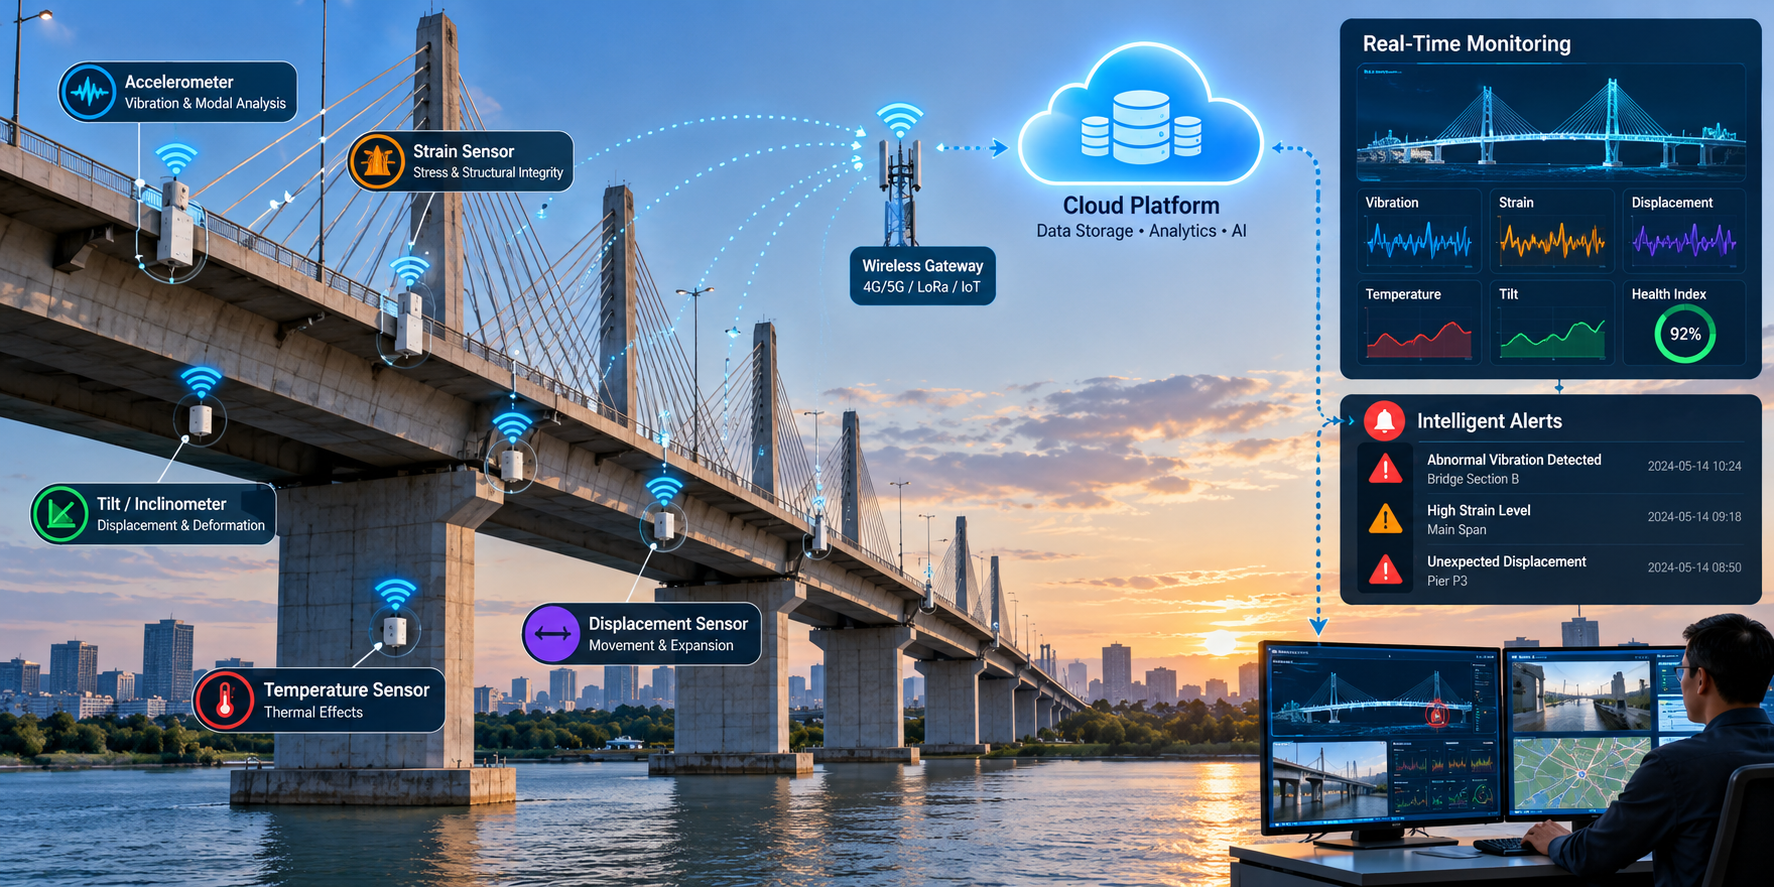
\includegraphics[width=\linewidth]{figures/ch11/ch11-02-v1-vague.png}};
\begin{scope}[x={(img.south east)},y={(img.north west)}]
  \tikzset{issuemark/.style={draw=Ch11IssueRed,line width=0.9pt,rounded corners=2pt,fill=white,fill opacity=0.90,text opacity=1,text=Ch11IssueRed,font=\sffamily\bfseries\scriptsize,inner sep=1.5pt}}
  \node[issuemark] at (0.35,0.62) {S1};
  \node[issuemark] at (0.24,0.82) {S2};
  \node[issuemark] at (0.55,0.84) {S3};
  \node[issuemark] at (0.95,0.64) {S4};
  \node[issuemark] at (0.78,0.44) {S5};
  \node[issuemark] at (0.64,0.76) {S6};
  \node[issuemark] at (0.62,0.28) {R1};
  \node[issuemark] at (0.64,0.91) {R2};
  \node[issuemark] at (0.11,0.56) {V1};
\end{scope}
\end{tikzpicture}
\caption{一句模糊提示词得到的初稿（反例）。编号对应表~\ref{tab:ch11-01} 的问题单：S1--S6 为科学错误，R1--R2 为阅读障碍，V1 为视觉一致性问题。科学错误超过三条时，修改单的第一项是重写输入，而不是修补这张图。底图由图像模型生成，其中文字为模型生成，未经核对。}\label{fig:ch11-02}
\end{figure}

\begin{table}[htbp]\centering\footnotesize
\setlength{\tabcolsep}{3pt}
\renewcommand{\arraystretch}{1.15}
\caption{将图~\ref{fig:ch11-02} 的“有点乱、不够专业”拆解为三层 9 条具体问题。}\label{tab:ch11-01}
\begin{tabularx}{\linewidth}{@{}c>{\raggedright\arraybackslash}p{17mm}>{\raggedright\arraybackslash}p{22mm}YY@{}}
\toprule
\textbf{编号} & \textbf{层级} & \textbf{位置} & \textbf{观察到的现象} & \textbf{为什么是问题} \\
\midrule
S1 & 科学错误 & 全桥构型 & 画成 6 塔三维透视斜拉桥，非双塔二维侧视图 & 与研究设定的双塔斜拉桥架构及立面工程制图不符 \\
S2 & 科学错误 & 桥上传感器 & 仅 5 个标签框；缺塔顶风速仪与 GNSS；应变计指在拉索上段而非主梁下缘；温度计放在桥墩下部 & 传感器类别不全、无法对应 12 个节点，布设部位违背工程常规 \\
S3 & 科学错误 & 网关至云平台 & 无线网关与云平台之间的蓝色虚线两端均带箭头 & 将单向汇聚上传监测数据画成了含义不明的双向箭头 \\
S4 & 科学错误 & 右上监控面板 & 凭空画出五条实时波形曲线及“Health Index 92\%”圆环 & 方法架构图不含实测数据，更无单一“92\% 健康评分”依据 \\
S5 & 科学错误 & 右中报警面板 & 写出 2024-05-14 的三条具体报警（B 段振动、主跨高应变、P3 墩位移） & 捏造了监测日期、墩号与结构异常事件 \\
S6 & 科学错误 & 全图文字框 & 英文标题、副标题、通信协议名与数值直接烧录在像素图中 & 文字属科学内容，锁死在位图中无法后期编校或改为中文 \\
R1 & 阅读障碍 & 背景与右下角 & 晚霞、城市天际线、江面反光与双屏操作员占据大半画幅 & 写实背景与装饰面板喧宾夺主，淹没传感与传输主干 \\
R2 & 阅读障碍 & 云平台内部 & 云朵内仅画数据库圆柱与“Data Storage $\cdot$ Analytics $\cdot$ AI” & 缺少“数据清洗 $\rightarrow$ 特征提取 $\rightarrow$ 阈值/异常判断”三步流程框 \\
V1 & 视觉一致性 & 传感器与标签 & 桥上节点全为同款白盒，说明框内却用蓝、橙、绿、红、紫五色圆图标 & 传感器本体无形状与颜色区分，不读文字无法按类型识别 \\
\bottomrule
\end{tabularx}
\end{table}

这张初稿仅第一层科学错误就有 6 条（S1--S6）。\textbf{当科学错误达到或超过三条时，修改单的第一条指令不是修补原图，而是退回任务书重写输入、重新生成。}

\section{修改单怎么写：一条只做一件事}

重新生成结构基准图（V2）前，先把系统构件、传感器数量与传输线定义为验收基准（表~\ref{tab:ch11-02}）。

\begin{table}[htbp]\centering\footnotesize
\setlength{\tabcolsep}{3pt}
\renewcommand{\arraystretch}{1.15}
\caption{斜拉桥结构健康监测系统示意图的对象表与关系表（V2 起的验收基准）。}\label{tab:ch11-02}
\begin{tabularx}{\linewidth}{@{}l>{\raggedright\arraybackslash}p{25mm}c>{\raggedright\arraybackslash}p{36mm}Y@{}}
\toprule
\textbf{编号} & \textbf{对象或关系} & \textbf{数量} & \textbf{位置（侧视图）} & \textbf{图形与线型约定（无字底图）} \\
\midrule
B1--B2 & 主梁与桥塔 & 1 梁 2 塔 & 左 $70\%$；塔在 $x\approx 0.22, 0.50$ & 浅灰扁长条主梁；中灰竖直单柱塔 \\
B3 & 斜拉索 & 16 & 每塔两侧各 4 根，扇形连塔上部与主梁 & 深灰细直线，全部连塔与梁，不入水不接地 \\
B4--B5 & 桥墩与水面 & 4 墩 1 水带 & 两塔下基础 + 两端边墩；底部水带 & 灰色墩座；浅蓝水面带 \\
S1--S5 & 加速度计 & $3+2$ & 主跨 $1/4, 1/2, 3/4$ 桥面（3）+ 两塔最长外索中部（2） & 蓝色小方块（每个传感器旁附 1 个黑点表示无线节点 N） \\
S6--S7 & 应变计 & 2 & 主跨跨中梁底、左塔旁梁底 & 绿色小矩形 \\
S8 / S9 & 风速仪 / GNSS & 各 1 & 左塔塔顶（S8）/ 右塔塔顶（S9） & 风杯形小图标 / 小圆盘天线图标 \\
S10 / S11--S12 & 温度计 / 位移计 & $1 / 2$ & 左边跨桥面（1）/ 两端伸缩缝（2） & 小圆形温度计图标 / 紫色小方块 \\
G / C / P / D & 网关/云/处理/终端 & 1/1/3/1 & 右 $30\%$ 数据路径区 & 右岸机柜加天线（G）；云内服务器条与三串联空框（C、P）；最右显示器加手机（D） \\
L1 & 无线传输 & 多条 & 各传感器节点 N $\rightarrow$ 网关 G & 橙色短虚线加小波纹，必须与斜拉索明显不同 \\
L2 / L3 / L4 & 上传 / 处理 / 预警 & 1 / 2 / 1 & G$\rightarrow$C / P 三框间 / P 末框$\rightarrow$D & 橙色实线箭头 / 深灰小箭头 / 红色实线箭头（全图唯一红色） \\
\bottomrule
\end{tabularx}
\end{table}

在 \scidraw{} 科研绘图向导（\sdtool{figure-workflow}）中选择“机制与流程图”路线，把模板替换为以下任务书并下载保存，再到流程图入口（\sdtool{workflow-diagram-generator}）或提示词绘图（\sdtool{ai-drawing}）生成：

\begin{Prompt}
【用途与读者】硕士论文第 2 章方法部分的系统示意图；印刷宽度约 160 mm（单页通栏），
读者为土木与结构工程同行。
【目标】让读者看清：传感器布设在桥的哪些部位、测什么；数据如何经无线节点到
现场网关、再上传云端分析；预警如何送达管理人员。
【材料】Farrar & Worden 2007；Ko & Ni 2005；Lynch & Loh 2006。本图为教学用简化架构，
不对应某座真实桥梁，不含任何监测数据。
【对象】见对象表 B1–B5、S1–S12、G、C、P、D；斜拉索每塔每侧 4 根，共 16 根；
传感器共 12 个，同类传感器同形同色。
【关系】L1 无线传输：橙色短虚线带小波纹，从各传感器到网关，不得与斜拉索相似；
L2 网关→云：橙色实线箭头；L3 云内三步处理：深灰小箭头；L4 判断→终端：红色箭头，
全图唯一红色。
【布局】横向 2:1。左 70% 为桥的侧视图（水面在下），右 30% 自下而上为网关、云、
终端；数据从左到右、自下而上流动。底部 10% 留给图例。
【视觉】白底，扁平二维工程示意风格，无渐变、无阴影、无 3D；结构灰阶，传感器用蓝/绿/紫。
【限制】底图不含任何文字、字母、数字；不画车辆、行人、城市、数据曲线、裂缝、主缆；
不画从云到传感器或从传感器到终端的直接箭头。
【验收】双塔斜拉桥；拉索 16 根连塔与梁；12 个传感器位置与类型正确；L1–L4 方向正确；
无线虚线与拉索可区分；底图无文字；160 mm 宽时图标可辨。
\end{Prompt}

转为结构化英文提示词提交生成（完整提示词见本书仓库 \texttt{cases/} 目录，关键段落如下）：

\begin{Prompt}
Flat 2D engineering schematic, landscape 2:1, pure white background, clean vector
style, flat fills, thin dark gray outlines, no gradients, no shadows, no 3D.
ABSOLUTELY NO TEXT: no letters, words, numbers, symbols, labels, legend or title.
LEFT 70% - SIDE VIEW OF A TWIN-PYLON CABLE-STAYED BRIDGE (no main cable, no hangers):
- Pale blue water band (y 0.75-0.88); light gray deck girder (x 0.03-0.68, y 0.60-0.63);
  two medium gray vertical pylons at x 0.22 and x 0.50 on gray piers; two end piers.
- Exactly 16 straight thin dark gray stay cables: 4 left and 4 right on each pylon,
  every cable connecting pylon to deck, none touching water or ground.
- SENSORS (12 total, each with a tiny black wireless node dot beside it):
  3 blue squares on main-span deck (1/4, 1/2, 3/4); 2 blue squares on longest outer
  cables; 2 green rectangles under deck; 1 cup anemometer on left pylon top; 1 dish
  GNSS antenna on right pylon top; 1 round thermometer on left side span; 2 purple
  squares at both deck ends.
RIGHT 30% - DATA PATH: gateway cabinet with antenna on right bank; cloud outline with
3 server bars and 3 empty rounded processing boxes connected by dark gray arrows;
operator terminal (monitor + phone) at far right.
LINES: short orange dashed wireless lines with wave marks from sensors to gateway;
one solid orange upload arrow (gateway -> cloud); one solid red alert arrow (last box
-> terminal; red used nowhere else). Keep bottom 10% empty for legend.
\end{Prompt}

把同一英文提示词连续生成三次，每次放大到 $200\%$ 对照表~\ref{tab:ch11-02} 清点：第 1 次生成中，每塔每侧连到塔身的拉索只有 $3+3+3+3=12$ 根，左外侧蓝色传感器附着在一段上端悬空的孤立斜线上，淘汰；第 3 次生成虽有 16 条拉索走向和 12 个传感器，但主跨拉索交叉拥挤，左塔顶风速仪被涂成与加速度计相同的蓝色，网关悬空且云压入水面带，淘汰；第 2 次生成（图~\ref{fig:ch11-03}）具备双塔侧视、16 条连接塔与主梁的拉索走向、全部 12 个传感器及旁侧黑点、网关/云/处理框/终端与四类箭头的正确方向，且全图零文字，选作后续比较的\textbf{候选结构基准（V2）}。

\begin{figure}[htbp]\centering
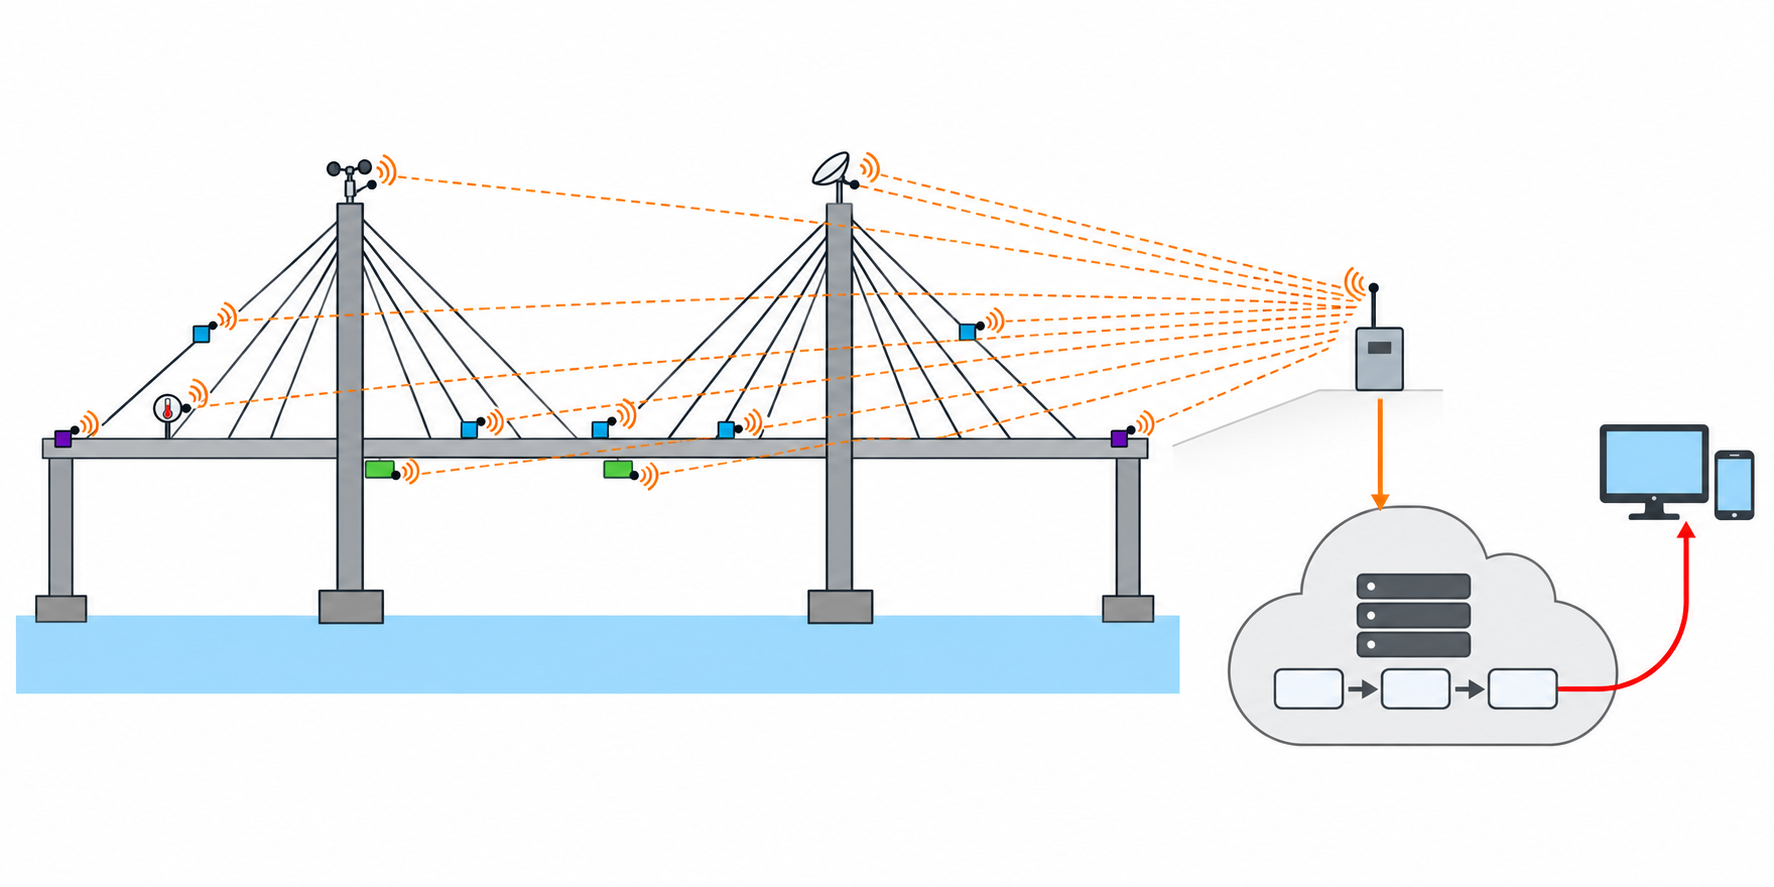
\includegraphics[width=\linewidth]{figures/ch11/ch11-03-v2-brief.png}
\caption{按完整任务书生成的候选结构基准 V2（第 2 次生成结果）。桥型、16 条斜拉索走向、12 个传感器、右侧子系统与数据流语义方向符合表~\ref{tab:ch11-02}，全图无文字，作为后续所有版本比较的参考基准；但仍留有无线虚线偏细、云在网关下方、温度计内部带红色、图标偏小及拉索局部白隙等缺陷（见表~\ref{tab:ch11-03} 修改单）。底图由图像模型生成。}\label{fig:ch11-03}
\end{figure}

V2 只是比较基准而非验收通过的终稿。对照任务书对其全面体检，即可写出结构化\textbf{修改单}（表~\ref{tab:ch11-03}）。每条修改单包含编号、层级、位置、实测现象、修改要求、**必须保持不变的内容**、核对方法与执行通道。

\begin{table}[htbp]\centering\footnotesize
\setlength{\tabcolsep}{3pt}
\renewcommand{\arraystretch}{1.15}
\caption{针对候选基准 V2（图~\ref{fig:ch11-03}）实测问题编写的修改单。}\label{tab:ch11-03}
\begin{tabularx}{\linewidth}{@{}c>{\raggedright\arraybackslash}p{14mm}>{\raggedright\arraybackslash}p{18mm}YYY>{\raggedright\arraybackslash}p{18mm}@{}}
\toprule
\textbf{ID} & \textbf{层级} & \textbf{位置} & \textbf{实测现象与影响} & \textbf{修改要求} & \textbf{必须保持不变} & \textbf{执行通道} \\
\midrule
R2 & 阅读障碍 & 传感器至网关线 & 橙色无线虚线偏细，横穿拉索扇面时区分度不足 & 改为更粗的橙色短虚线并带波纹，与深灰细实线拉索明显不同 & 桥型、16 条拉索、12 个传感器、网关/云/终端及 L2--L4 & 生成模型（参考图修改）；失败两次则改用 TikZ \\
R3 & 阅读障碍 & 全部传感器 & $160\ \text{mm}$ 宽下蓝方块约 $1.44\text{--}1.80\ \text{mm}$，小于 $2\ \text{mm}$ & 传感器图标放大约 $1.5$ 倍（与 R2 分开独立执行） & 同上全部结构与连接线 & 生成模型（独立轮次）或排版层覆盖 \\
R4 & 阅读障碍 & 右侧数据路径 & 网关在上方（$y\approx 0.41$）、云在下方（$y\approx 0.71$），上传箭头朝下，路径折返 & 教学稿按实测位置叠字说明；正式投稿需对调网关与云的上下位置 & 左 $70\%$ 桥体、16 根拉索与 12 个传感器不变 & 排版层适配坐标或重生成右侧 \\
V1 & 视觉一致性 & 温度计与蓝方块 & 温度计含红色液柱，违反“红色仅用于预警”；蓝方块色值未精确统一 & 温度计去红改灰；同类加速度计统一色值（如 \texttt{\#4C78A8}） & 其余传感器、结构灰阶与红预警箭头 & 后期图像/排版层修色 \\
V2 & 视觉一致性 & 拉索交界与水面 & 部分拉索穿过图标和波纹处有白色断开窄隙；水面与屏幕带渐变 & 正式发表前在矢量或图像软件中补连拉索断口、平涂渐变区 & 16 条拉索端点与传感器坐标 & 排版层 / 矢量软件 \\
T1 & 文字与图例 & 全图与底边 & 底图无文字，需构件名、子系统名与图例 & 在 LaTeX/TikZ 中按实测坐标叠加 7 处标签与底部图例 & 底图像素不动 & 排版层（TikZ） \\
\bottomrule
\end{tabularx}
\end{table}

\begin{BookNote}
\textbf{修改单的三条规则：}（1）\textbf{一次只改一类问题}，不把加粗虚线、放大图标、对调位置塞进同一条生成指令；（2）\textbf{必须写明“保持不变”清单}，用具体对象和数量取代笼统的“其余不变”；（3）\textbf{文字、精确色值、断口补线与对齐优先在排版层完成}，不靠生成模型反复重绘。
\end{BookNote}

\section{局部指令的连带变化：怎么发现它}

为什么修改单如此谨慎地限制生成模型修改？因为图像生成模型的“局部修改”并不是在原图图层上擦改一根线，而是以参考图和提示词为条件**重新合成整张画布**。在 \scidraw{} 绘图（\sdtool{ai-drawing}）中选择历史图作为参考图修改时，同样没有“对象锁定”或“区域像素冻结”，模型可能顺手改动未提及的对象——即发生\textbf{连带变化（collateral changes）}。

\subsection{真实例子一：第 7 章只要求统一风格，却改坏了五处结构}

先看本书第 7 章胰岛素促进 GLUT4 转位机制图的真实迭代记录（图~\ref{fig:ch11-07}）。其 V2 基准图（图~\ref{fig:ch11-07}左）已画对 13 个对象、6 枚琥珀色磷酸化圆点及五类线型。进入 V3 时，作者只要求统一蛋白蓝色色值、统一线宽并增加留白，提示词写明“保持相同内容与布局”。

然而，当第 1 次生成未传入 V2 参考图、仅凭修订提示词重新生成时（图~\ref{fig:ch11-07}中），虽然配色和线条变得干净，却出现了五处严重的结构连带变化：(a) 受体、IRS-1、Akt 和 AS160 上的 6 枚磷酸化圆点全部丢失；(b) 胰岛素由 3 珠减为 2 珠且脱离受体；(c) 原本紧贴质膜内叶的 PDK1 与 Akt 脱离质膜掉入胞质；(d) PI3K 与 PDK1 之间多出一条未经授权的实心激活箭头；(e) 每个囊泡上的 GLUT4 由 1 个变为多个，胞内还多出葡萄糖六边形。直到第 2 次将 V2 作为参考图传入（图~\ref{fig:ch11-07}右），才保住了主要结构与磷酸化圆点。即便传入参考图，第 7 章做配色反例实验时，模型仍在重绘中把 $\text{PIP}_2 \rightarrow \text{PIP}_3$ 转化弧的空心箭头悄悄改成了实心箭头。

\begin{figure}[htbp]\centering
% FIG ch11-07 Chapter 7 collateral reuse (Chinese)
\usetikzlibrary{arrows.meta,calc}
\begin{tikzpicture}
  \def\panelW{0.31\linewidth}
  \definecolor{Ch11AnnotRed}{HTML}{C0392B}
  \node[anchor=south west, inner sep=0] (imA) at (0,0) {%
    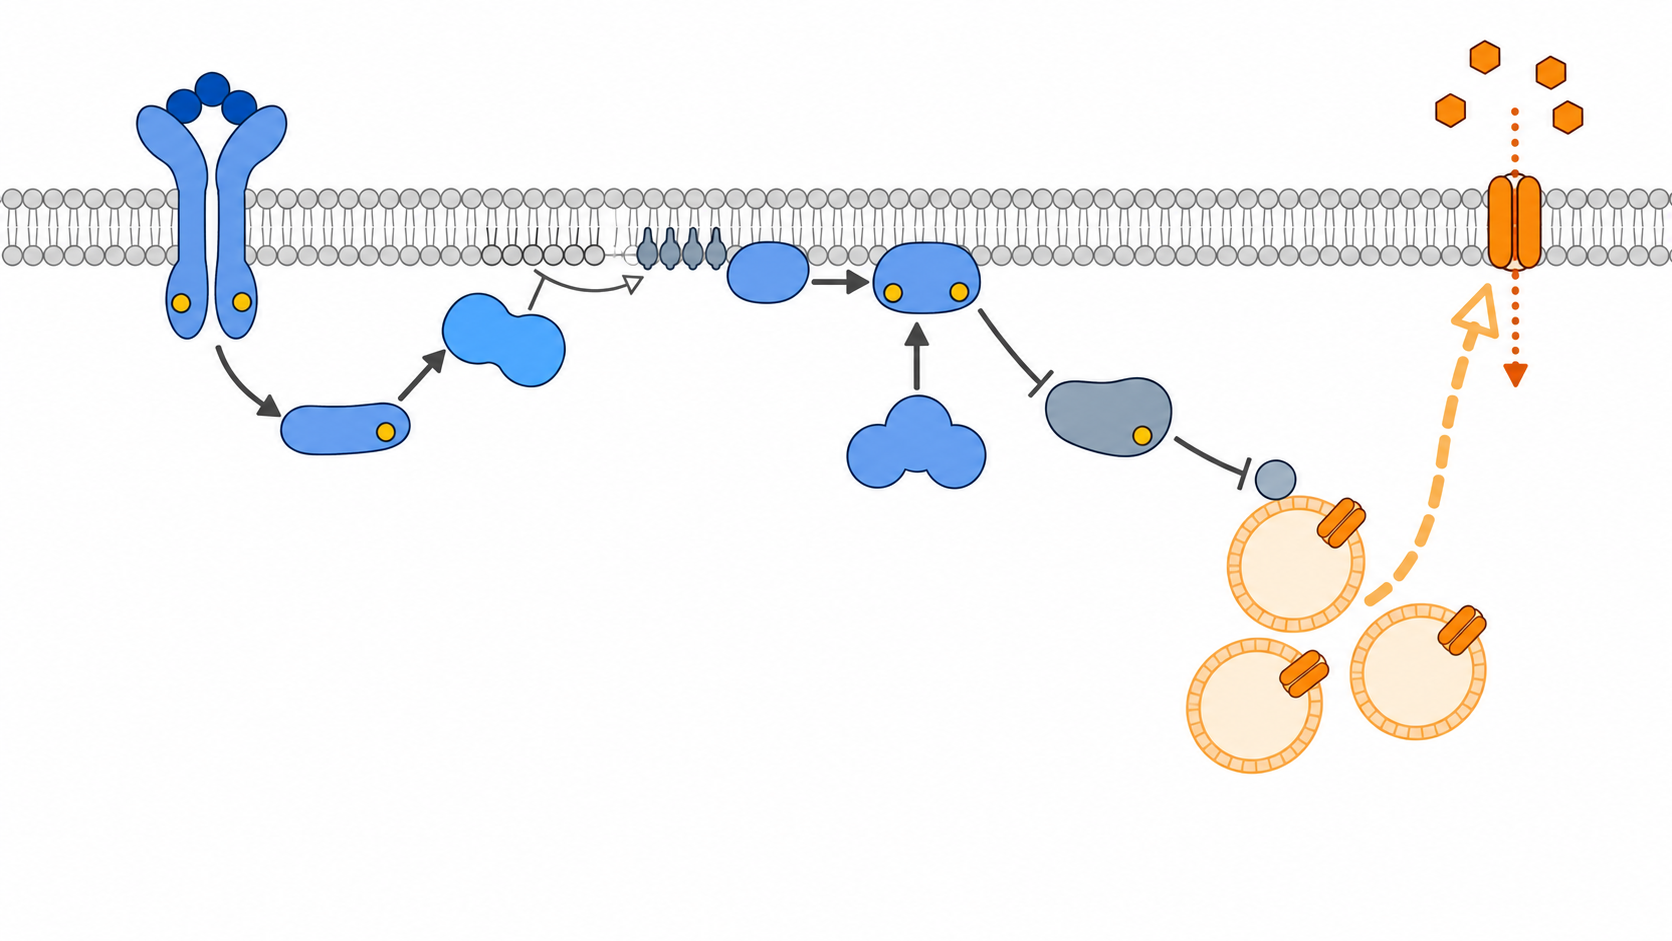
\includegraphics[width=\panelW]{figures/ch11/ch11-07a-ch07-v2.png}};
  \node[font=\small\sffamily, anchor=south] at ($(imA.north)+(0,2mm)$) {V2 基准};

  \node[anchor=south west, inner sep=0] (imB) at (0.345\linewidth,0) {%
    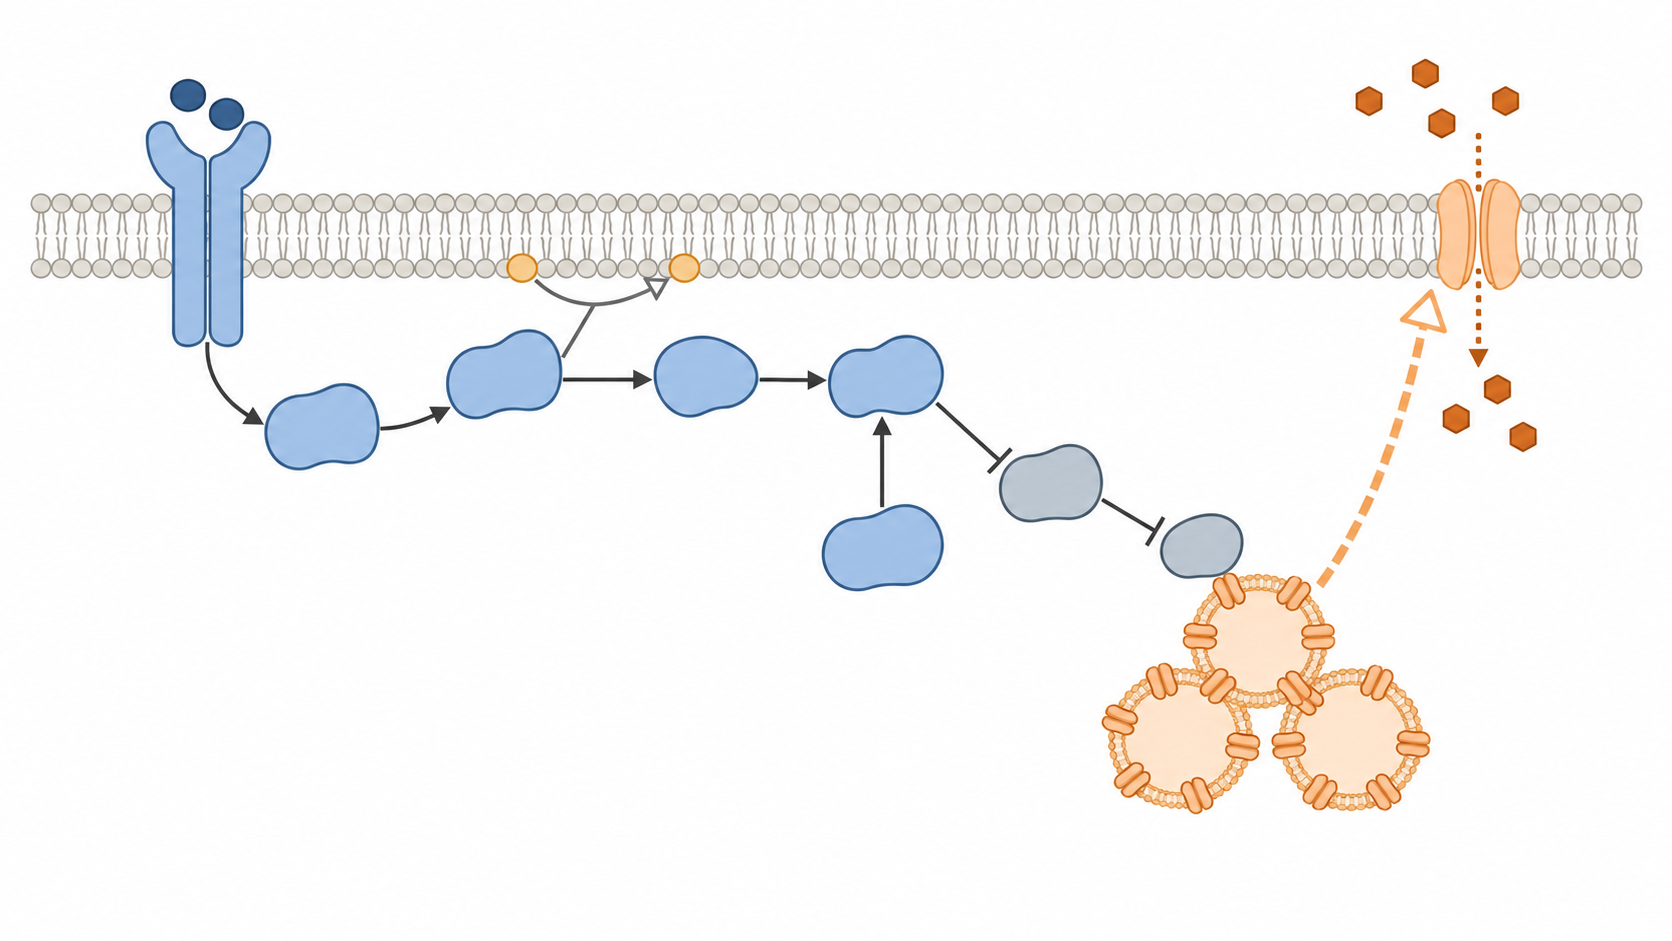
\includegraphics[width=\panelW]{figures/ch11/ch11-07b-ch07-v3-alt1.png}};
  \node[font=\small\sffamily, anchor=south] at ($(imB.north)+(0,2mm)$) {V3 第 1 次（不采用）};
  \begin{scope}[x={(imB.south east)},y={(imB.north west)}]
    \draw[Ch11AnnotRed, line width=0.7pt] (0.11,0.28) circle (0.035);
    \node[font=\scriptsize\sffamily, text=Ch11AnnotRed, anchor=west] at (0.15,0.28) {(a)};
    \draw[Ch11AnnotRed, line width=0.7pt] (0.10,0.08) circle (0.04);
    \node[font=\scriptsize\sffamily, text=Ch11AnnotRed, anchor=west] at (0.14,0.08) {(b)};
    \draw[Ch11AnnotRed, line width=0.7pt] (0.48,0.38) circle (0.06);
    \node[font=\scriptsize\sffamily, text=Ch11AnnotRed, anchor=west] at (0.54,0.38) {(c)};
    \draw[Ch11AnnotRed, line width=0.7pt] (0.34,0.36) circle (0.045);
    \node[font=\scriptsize\sffamily, text=Ch11AnnotRed, anchor=west] at (0.39,0.36) {(d)};
    \draw[Ch11AnnotRed, line width=0.7pt] (0.76,0.70) circle (0.07);
    \node[font=\scriptsize\sffamily, text=Ch11AnnotRed, anchor=west] at (0.82,0.70) {(e)};
  \end{scope}

  \node[anchor=south west, inner sep=0] (imC) at (0.69\linewidth,0) {%
    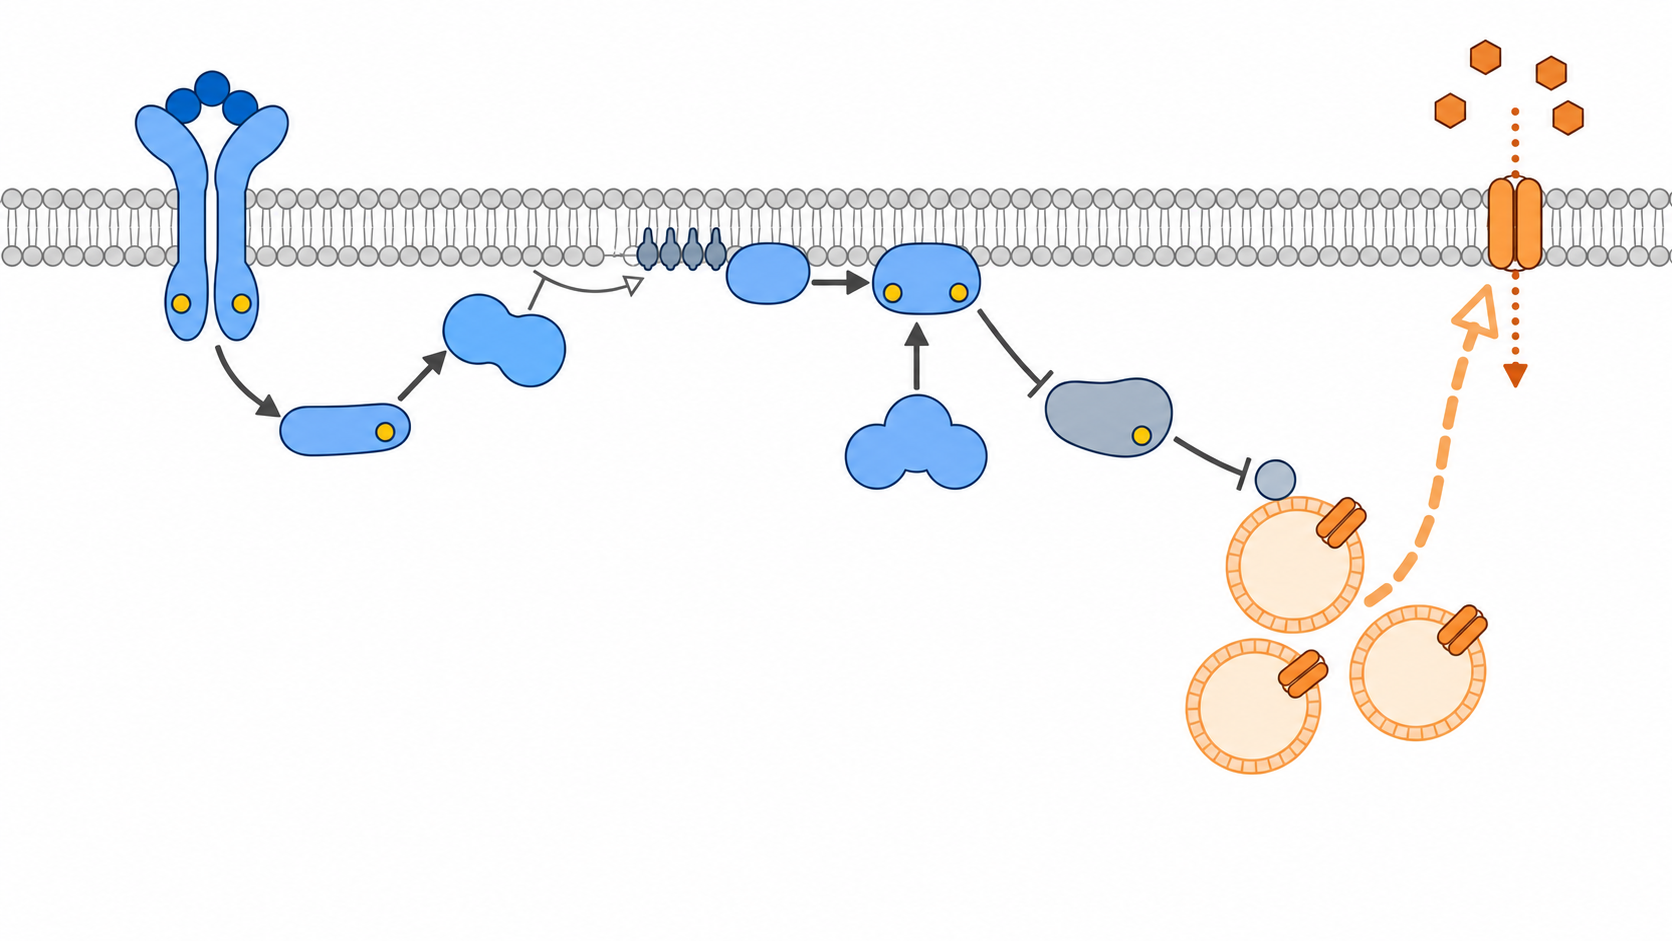
\includegraphics[width=\panelW]{figures/ch11/ch11-07c-ch07-v3.png}};
  \node[font=\small\sffamily, anchor=south] at ($(imC.north)+(0,2mm)$) {V3 第 2 次（采用）};
\end{tikzpicture}

\caption{第 7 章的真实迭代：关于配色与线型的修订提示词也可能改动结构。左为 V2 基准；中为同一修订提示词第 1 次生成（未传参考图）：(a) 磷酸化标记全部丢失，(b) 胰岛素由三珠变两珠且脱离受体，(c) PDK1 与 Akt 离开质膜，(d) 新增未要求的 PI3K$\rightarrow$PDK1 激活箭头，(e) 每个囊泡上的 GLUT4 由一个变为多个；右为传入 V2 作参考图的第 2 次生成，主要结构保留，但仍需整图复核。三图均由图像模型生成。}\label{fig:ch11-07}
\end{figure}

\subsection{真实例子二：本章 V3 参考图修改的三次实测}

再看本章修改单第一项（R2）。在 \scidraw{} 绘图中从历史记录选择 V2（图~\ref{fig:ch11-03}）作为参考图，输入只改无线传输线的指令：

\begin{Prompt}
把所有从传感器到网关的无线传输线改为更粗的橙色短虚线，并在线上加小波纹，
让它们与斜拉索一眼就能区分。其他内容保持不变。
\end{Prompt}

实际提交的英文指令为：

\begin{Prompt}
Using the reference image, change only the wireless lines from the sensors to
the gateway: make them thicker orange short-dashed lines with small wave marks,
so they cannot be confused with the stay cables. Keep everything else
unchanged. No text.
\end{Prompt}

我们独立以 V2 为参考图连续执行了三次修改，每次都按表~\ref{tab:ch11-02} 清点全部对象。图~\ref{fig:ch11-04} 将 V2（左）与 V3 第 1 次结果（右）并排对比。

\begin{figure}[htbp]\centering
\resizebox{\linewidth}{!}{%
\begin{tikzpicture}
\definecolor{Ch11OkGreen}{HTML}{2E8B57}
\definecolor{Ch11WarnRed}{HTML}{C0392B}
\node[anchor=south west,inner sep=0] (imL) at (0,0) {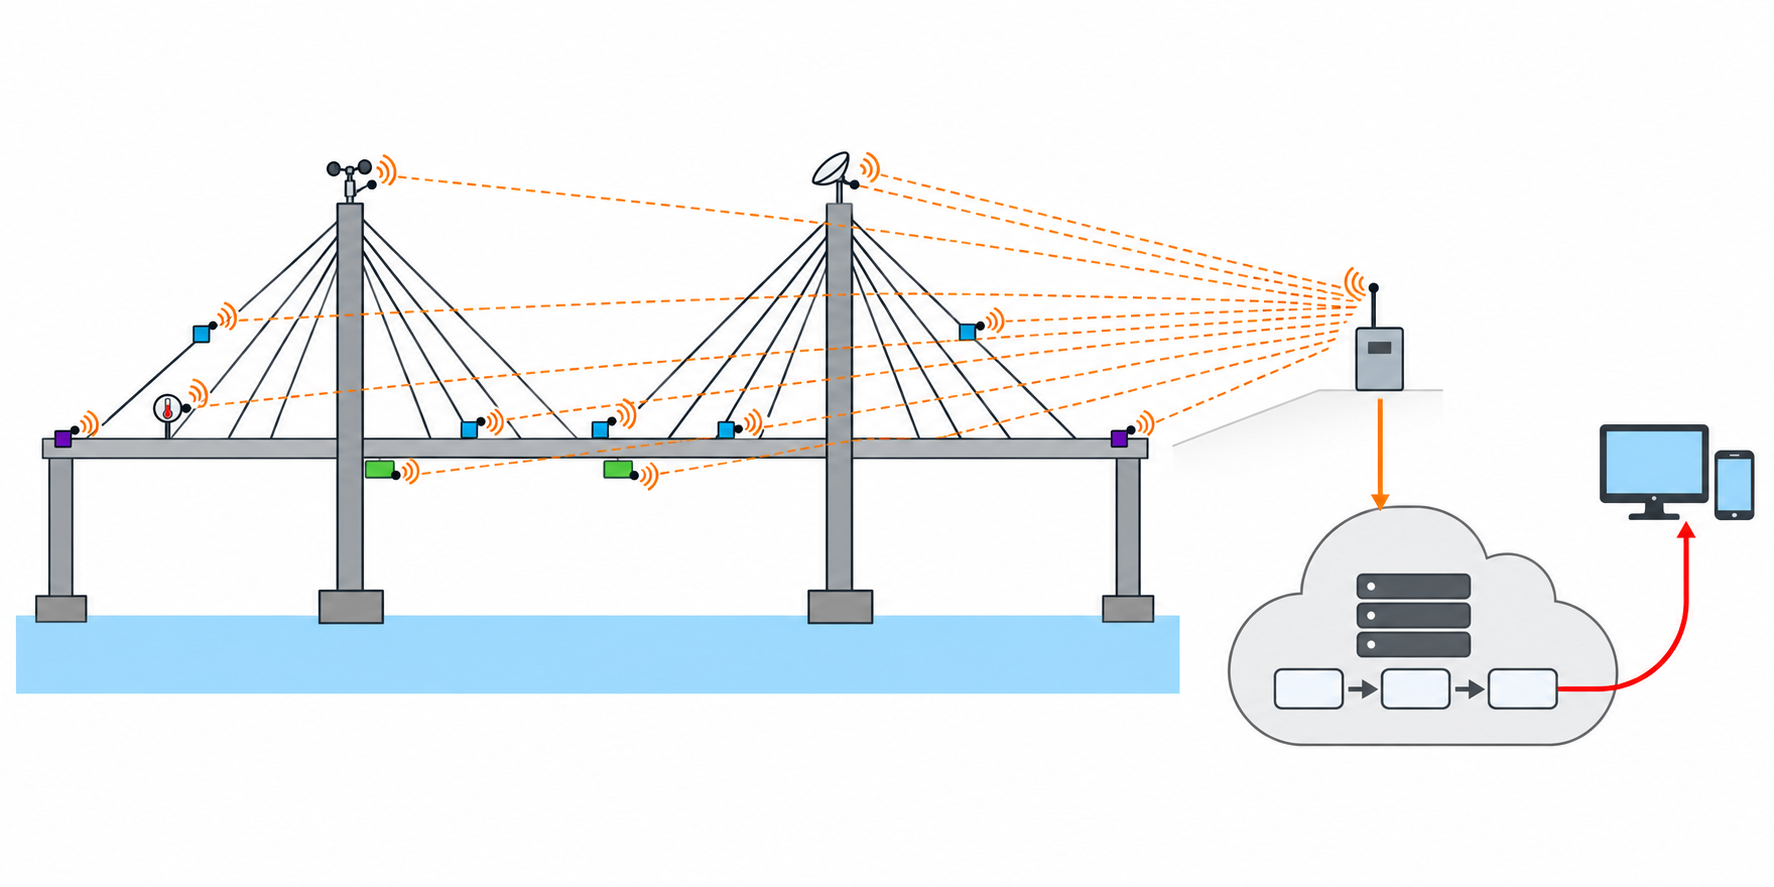
\includegraphics[width=0.488\linewidth]{figures/ch11/ch11-03-v2-brief.png}};
\node[font=\sffamily\footnotesize,anchor=south] at ($(imL.north)+(0,1.5mm)$) {V2 候选基准（修改前）};
\node[anchor=south west,inner sep=0] (imR) at (0.512\linewidth,0) {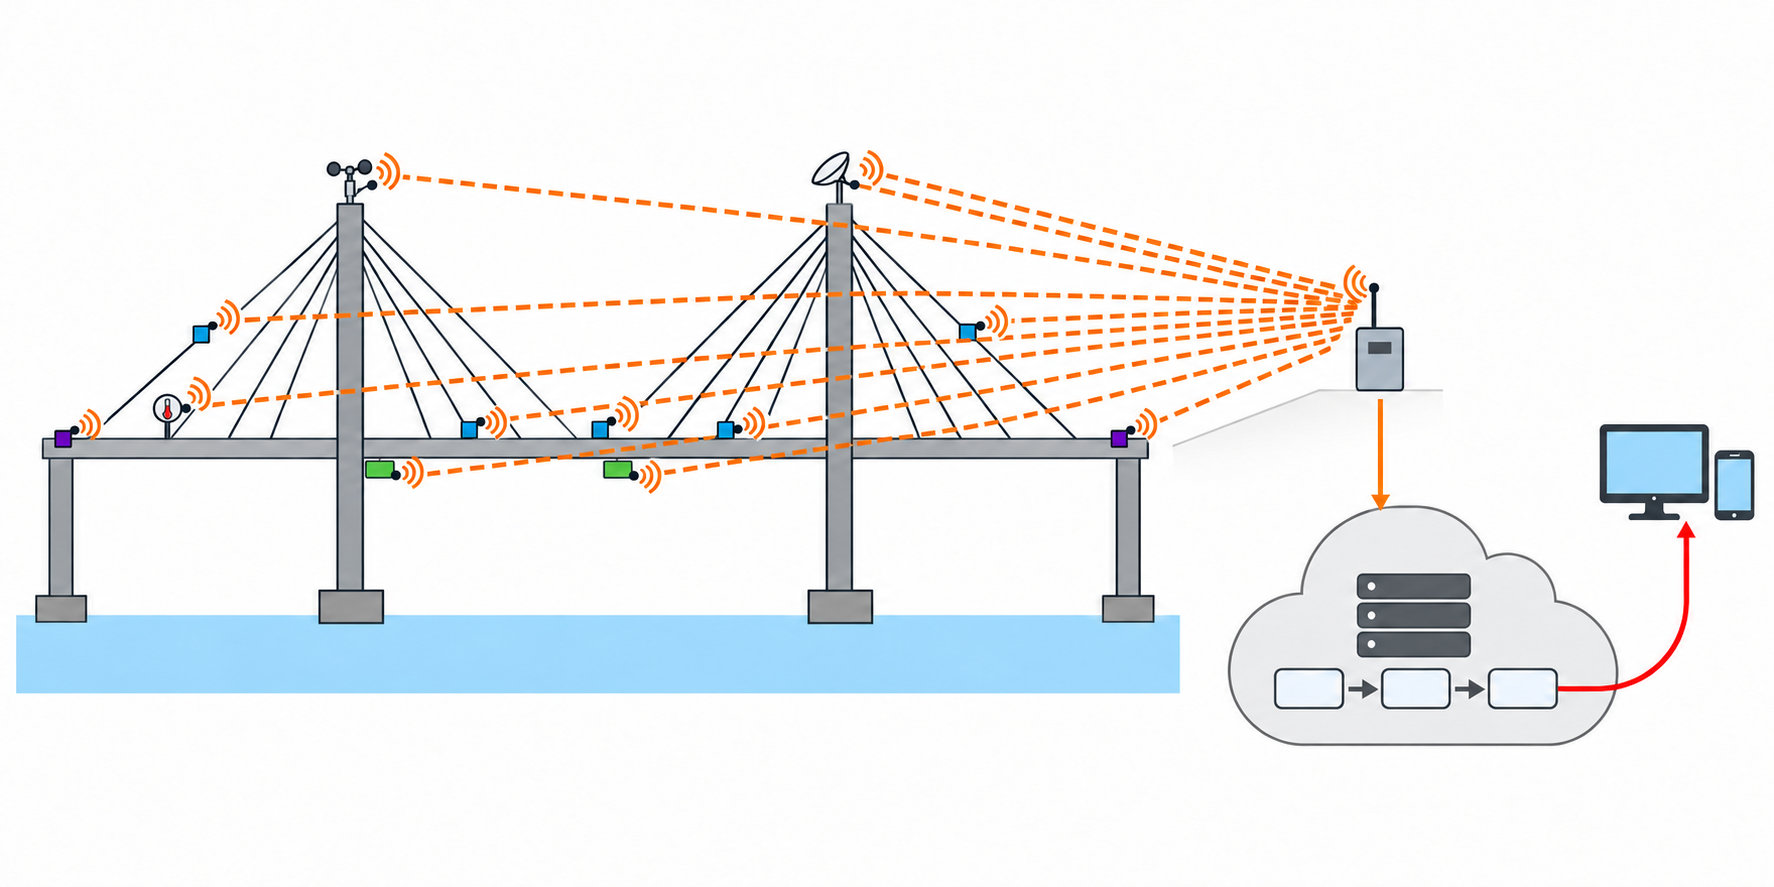
\includegraphics[width=0.488\linewidth]{figures/ch11/ch11-04-v3-collateral.png}};
\node[font=\sffamily\footnotesize,anchor=south] at ($(imR.north)+(0,1.5mm)$) {V3 第 1 次（参考图局部修改后）};
\begin{scope}[x={(imR.south east)},y={(imR.north west)}]
  \draw[Ch11OkGreen,line width=0.9pt,rounded corners=2pt] (0.50,0.61) rectangle (0.76,0.80);
  \node[fill=white,fill opacity=0.9,text opacity=1,text=Ch11OkGreen,font=\sffamily\bfseries\scriptsize,inner sep=1pt,anchor=south] at (0.63,0.81) {目标修改完成：橙虚线加粗};
  \draw[Ch11WarnRed,dashed,line width=0.7pt,rounded corners=2pt] (0.06,0.49) rectangle (0.13,0.59);
  \node[fill=white,fill opacity=0.9,text opacity=1,text=Ch11WarnRed,font=\sffamily\scriptsize,inner sep=1pt,anchor=south] at (0.10,0.60) {继承偏差 1};
  \draw[Ch11WarnRed,dashed,line width=0.7pt,rounded corners=2pt] (0.68,0.14) rectangle (0.91,0.44);
  \node[fill=white,fill opacity=0.9,text opacity=1,text=Ch11WarnRed,font=\sffamily\scriptsize,inner sep=1pt,anchor=north] at (0.80,0.13) {继承偏差 2：云仍在网关下方};
\end{scope}
\end{tikzpicture}}
\caption{只要求修改无线传输线后得到的 V3 第 1 次结果（右），与候选基准 V2（左）并排。绿色实线框标出已完成的目标修改（橙色短虚线加粗、波纹更醒目）；三次独立参考图修改均保住了 16 条斜拉索走向与 12 个传感器，未观察到明显结构连带变化，但仍需整图复核。红色虚线框标出从 V2 原样继承的既有偏差（温度计带红色、云在网关下方）。底图均由图像模型生成，未经人工改动。}\label{fig:ch11-04}
\end{figure}

三次实测给出了三点结论：（1）\textbf{目标修改完成}：三次尝试都把橙色短虚线明显加粗、节点旁波纹更醒目，与深灰细实线拉索清楚区分（但波纹仍集中在节点旁，未遍布链路中段）；（2）\textbf{三次尝试均未出现少索、少传感器或网关移位等结构连带变化}：2 座桥塔、16 条拉索走向、12 个传感器（$3+2+2+1+1+1+2$）和右侧网关、云、3 个处理框、终端及箭头全部保持一致；（3）\textbf{V2 原有缺陷被原样继承}：温度计带红（继承偏差 1）、云在网关下方（继承偏差 2）、小图标与拉索局部白隙在三次结果中依然存在。

这说明连带变化具有随机性：**“本次没有发生结构连带变化”只能在逐项清点后得出，绝不能在清点前假定。**

\subsection{用并排比较、像素差异图与对象计数表核验}

排查连带变化可结合三种方法（图~\ref{fig:ch11-05}）：

\begin{figure}[htbp]\centering
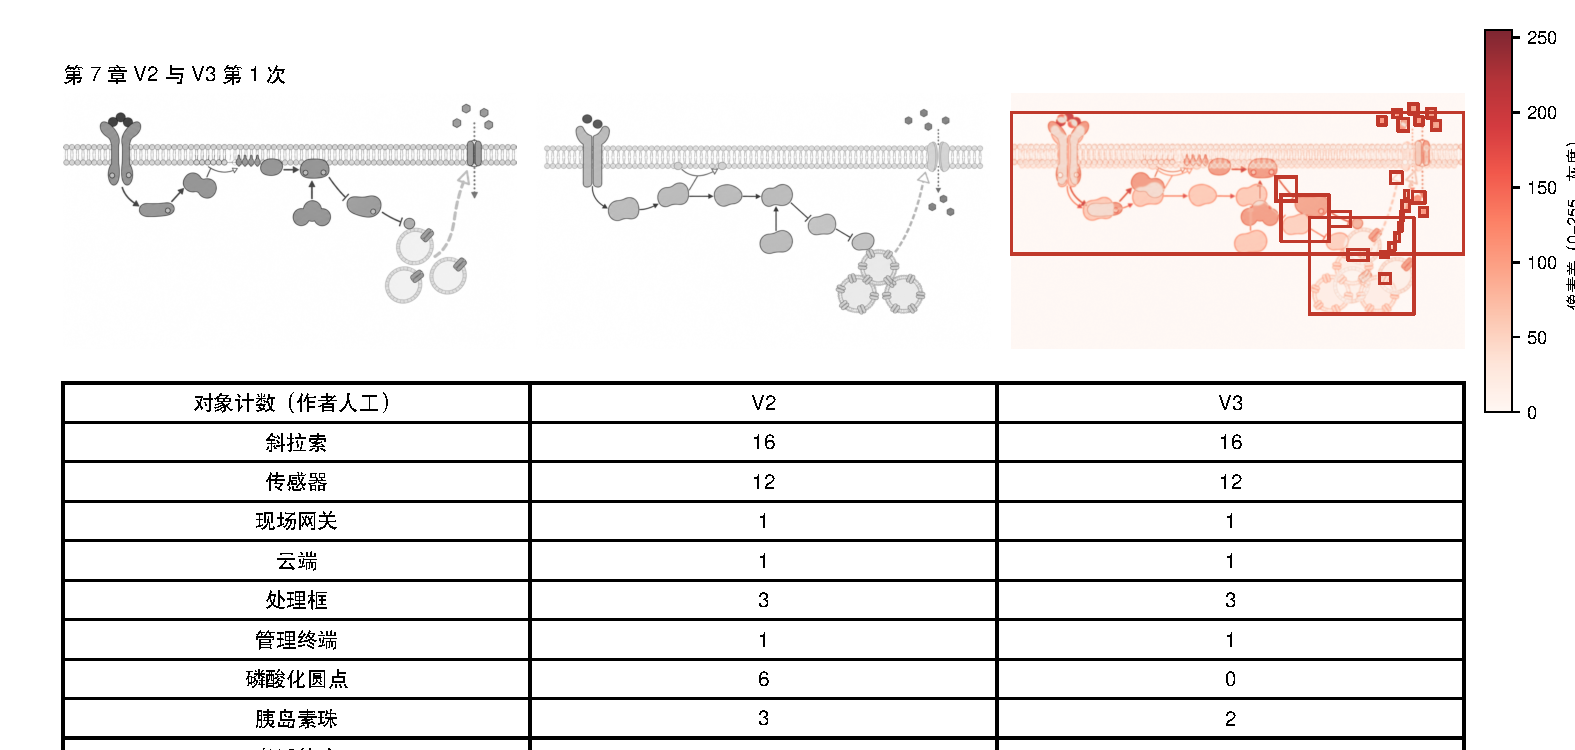
\includegraphics[width=\linewidth]{figures/ch11/ch11-05-diff-and-count-zh.pdf}
\caption{用差异图和对象计数发现连带变化。差异图显示两版之间灰度像素变化的位置；构图基本不变时，它能直接指出变动区；整张图被重排重绘时（上排：第 7 章 V2 与 V3 第 1 次尝试），差异红框遍布全图（共 24 个区域），此时只能依靠按对象表逐项计数（下表：前 6 行为本章 V2 与 V3 计数，后 4 行为第 7 章计数）。计数由作者人工完成。}\label{fig:ch11-05}
\end{figure}

第一，\textbf{同尺寸并排比较或叠放切换}。\scidraw{} 当前未内置版本并排对比视图，需将新旧两版下载后同宽并排（如图~\ref{fig:ch11-04}）或在看图软件中快速前后切换，靠视觉闪烁发现未修改区的位移。

第二，\textbf{像素差异热图及其局限}。将两图缩放到同尺寸转灰度（$0\text{--}255$），计算逐像素绝对差，经高斯模糊（半径约 2 像素）抑制抗锯齿噪点后，圈出灰度差大于 40 的连通域。当构图保持不变时，热图能直接指出变动线条；但当模型重排了全图构图时——如图~\ref{fig:ch11-05} 上排的第 7 章 V2 与 V3 第 1 次尝试——全图约 $14.6\%$ 的像素超阈值，24 个红框覆盖全图，失去定位能力。

第三，\textbf{人工对象计数表（最终防线）}。对照对象表逐项清点（图~\ref{fig:ch11-05} 下表）：本章 V2 与 V3 的斜拉索（16/16）、传感器（12/12）、网关（1/1）、云端（1/1）、处理框（3/3）、管理终端（1/1）完全一致；而第 7 章 V2 与 V3 第 1 次尝试中，磷酸化圆点由 6 变 0、胰岛素珠由 3 变 2、激活箭头由 4 变 5、每囊泡最大 GLUT4 由 1 变 3。像素差异图只作辅助，人工按表计数才能把住科学关。

\section{回到上一版再改，以及何时换走排版层}

一旦在某次修改中发现了连带变化（如丢了天线或少了拉索），绝不能在出错的 V3 上继续输入“把消失的天线加回来”。正如图~\ref{fig:ch11-08} 右下虚线框所示，在错误版本上叠加修改（$\text{V3} \rightarrow \text{V3}' \rightarrow \text{V3}''$）会让每次全图重绘引入新变形，错误层层累积且无法追溯。

\begin{figure}[htbp]\centering
\resizebox{\linewidth}{!}{\tikzset{every node/.append style={align=center}}% FIG ch11-08 version tree (Chinese)
\usetikzlibrary{arrows.meta,positioning,fit,calc}
\definecolor{Ch11BadRed}{HTML}{C0392B}
\definecolor{Ch11GoodGreen}{HTML}{2E8B57}
\providecommand{\ChElevenThumb}[2]{%
  \IfFileExists{#1}{%
    \includegraphics[width=24mm]{#1}%
  }{%
    \fbox{\parbox[c][16mm][c]{24mm}{\centering\scriptsize\sffamily #2\\{\tiny （底图待出）}}}}%
}
\begin{tikzpicture}[
  x=1mm, y=1mm,
  font=\sffamily\footnotesize,
  edge/.style={draw=BookInk!60, -{Stealth[length=2mm]}, line width=0.55pt},
  badedge/.style={draw=Ch11BadRed!70, dashed, -{Stealth[length=2mm]}},
  nlabel/.style={align=center, text width=26mm, font=\scriptsize},
]
  \node (V1) at (0,0) {\ChElevenThumb{figures/ch11/ch11-02-v1-vague.png}{V1}};
  \node[nlabel, below=1mm of V1] {模糊提示词};

  \node (V2) [below=14mm of V1] {\ChElevenThumb{figures/ch11/ch11-03-v2-brief.png}{V2\\基准}};
  \node[nlabel, below=1mm of V2] {\textbf{结构基准}};

  \node (V3) [below=14mm of V2] {\ChElevenThumb{figures/ch11/ch11-04-v3-collateral.png}{V3}};
  \node[nlabel, below=1mm of V3, text=Ch11BadRed] {连带变化\\{\tiny（不采用）}};

  \node (V4) at (42,-28) {\ChElevenThumb{figures/ch11/ch11-06-v4-recovered.png}{V4}};
  \node[nlabel, below=1mm of V4, text=Ch11GoodGreen] {回到 V2\\只改无线线};

  \node (Final) at (84,-28) {\ChElevenThumb{figures/ch11/ch11-06-v4-recovered.png}{终稿}};
  \node[nlabel, below=1mm of Final] {TikZ 标签与图例};

  \draw[edge] (V1) -- node[left, font=\tiny, align=right] {重写\\输入} (V2);
  \draw[edge] (V2) -- node[right=1.5mm, font=\tiny, align=left] {只改\\无线线} (V3);
  \draw[edge] (V2.east) -- node[above, font=\tiny] {只改无线线\\+ 保留清单} (V4.west);
  \draw[edge] (V4.east) -- node[above, font=\tiny] {叠加标签\\与图例} (Final.west);

  \node[draw=Ch11BadRed, dashed, rounded corners=2pt, inner sep=4pt, fit=(V3)] {};
  \node[font=\scriptsize, text=Ch11BadRed, right=1mm of V3] {×};

  \node (Vp1) at (42,-66) {\fbox{\parbox[c][16mm][c]{24mm}{\centering\scriptsize V3$'$\\示意}}};
  \node[font=\tiny, below=1mm of Vp1, text width=28mm, align=center] {把消失的天线加回来};
  \node (Vp2) [right=12mm of Vp1] {\fbox{\parbox[c][16mm][c]{24mm}{\centering\scriptsize V3$''$\\示意}}};
  \node[font=\tiny, below=1mm of Vp2, text width=28mm, align=center] {又一处变化};
  \draw[badedge] (Vp1) -- (Vp2);
  \node[draw=BookInk!40, dashed, rounded corners=2pt, inner sep=6pt,
    fit=(Vp1)(Vp2), label={[font=\scriptsize, yshift=2mm]above:错误做法：在错误版本上叠加}] {};
  \draw[badedge] (V3.east) -- ++(6,0) |- (Vp1.west);
\end{tikzpicture}
}
\caption{本章案例的版本树。当某次修改出现连带变化时不继续修补，而是回到基准 V2 另起分支 V4，重述保留清单后只改一件事。右下虚线框示意在错误版本上叠加修改时问题如何累积。（注：本章 V3 三次实测未发生构件丢失，图中 V3 分支用于示意出现连带变化时的标准回退逻辑。）}\label{fig:ch11-08}
\end{figure}

正确做法是在 \scidraw{} 历史记录中\textbf{重新选择基准 V2} 作为参考图，另起分支 V4，在指令中同时写明“只改一处”和“逐项保持不变清单”：

\begin{Prompt}
以这张图为准修改。只改一处：从传感器到网关的无线传输线，改为更粗的橙色短虚线并带小波纹。
必须保持不变（逐项）：
- 双塔斜拉桥侧视图，两座塔的位置、高度与形状不变；
- 斜拉索共 16 根：每座塔左右各 4 根，全部连接塔与主梁，位置与角度不变；
- 12 个传感器的位置、形状和颜色不变：主跨桥面 3 个蓝色方块、两根最长外侧索中部各 1 个蓝色方块、
  梁底 2 个绿色矩形、左塔顶风速仪、右塔顶 GNSS 天线、左边跨温度计、两端 2 个紫色方块；
- 网关、云、云内 3 个处理框、终端的位置不变；橙色上传箭头与红色预警箭头不变；
- 不添加任何新对象、新线或文字。如果无法在不改变其他内容的情况下完成，请保持原图不变。
\end{Prompt}

以 V2 为参考图执行该指令（英文同义改写见本书仓库）得到 V4 底图：无线短虚线显著加粗，16 条拉索走向与 12 个传感器全部保留，转灰度后粗虚线与细实线拉索仍清晰可分。

若某项局部修改附上保留清单后连续两次仍发生连带变化，就应\textbf{换走排版层路线}：例如将 V2 提示词中的无线线改为“不画任何从传感器到网关的连线（\texttt{Do not draw any lines from sensors to the gateway}）”，重新生成无无线链路的底图，核验 16 根拉索与 12 个传感器无误后，在 TikZ 中用代码绘制橙色虚线与波纹（代价是新底图仍需整图计数，好处是此后改线型不再触碰底图）。

与之相比，\scidraw{} 科学可视化（\sdtool{sci-vis}）中的数据图由代码或图表配置重绘，支持多轮对话修改及“恢复上一版/原版”，改配色或图例不会随机弄丢数据点；但数据图修改或恢复后同样需要整图复核，以防坐标轴范围裁掉极值或改变统计表达。

\section{修订记录、叠加终稿与整图复核}

每次迭代都应留下一行修订记录，写明基于哪一版、指令摘要、目标修改、意外变化或遗留偏差、复核结论及是否采用（表~\ref{tab:ch11-04}）。

\begin{table}[htbp]\centering\footnotesize
\setlength{\tabcolsep}{3pt}
\renewcommand{\arraystretch}{1.15}
\caption{本章斜拉桥监测示意图案例的逐版修订记录（按实测填写）。}\label{tab:ch11-04}
\begin{tabularx}{\linewidth}{@{}l>{\raggedright\arraybackslash}p{14mm}>{\raggedright\arraybackslash}p{22mm}YY>{\raggedright\arraybackslash}p{18mm}@{}}
\toprule
\textbf{版本} & \textbf{基于} & \textbf{指令摘要} & \textbf{目标修改与正面结果} & \textbf{实测偏差或意外变化} & \textbf{是否采用} \\
\midrule
V1（1 次） & — & 一句模糊英文提示词 & 生成写实大桥反例 & S1--S6 共 6 条科学错误（6 塔透视桥、缺风速仪/GNSS、双向箭头、虚构波形与 92\% 及报警等） & 否；重写输入 \\
V2 第 1 次 & 任务书 & 完整英文提示词 & 双塔侧视、12 个传感器、无文字 & $200\%$ 核对仅 12 根拉索连塔，左外侧有悬空孤立斜线段 & 否（备选 1） \\
V2 第 2 次 & 任务书 & 同一提示词第 2 次 & 16 条拉索走向、12 个传感器、子系统与四类箭头方向正确，无文字 & 无线线偏细；云在网关下方；温度计带红；图标偏小；拉索过图标处有窄白隙 & 选作比较基准 V2 \\
V2 第 3 次 & 任务书 & 同一提示词第 3 次 & 16 条拉索走向与 12 个传感器可辨 & 主跨拉索交叉拥挤；风速仪涂成蓝色；网关悬空；云压入水面带 & 否（备选 2） \\
V3（3 次） & V2 & 参考图修改：只加粗无线虚线并加波纹 & 三次均成功加粗橙色短虚线并强化节点旁波纹 & 三次均未发生少索或少传感器等结构连带变化；继承 V2 的云位置、红温度计与小图标偏差 & 选第 1 次作对比展示 \\
V4（1 次） & V2 & 回到 V2 + 只改无线线 + 逐项保留清单 & 无线虚线加粗完成，16 条拉索与 12 个传感器保持，灰度可区分 & 未引入新连带变化；仍继承 V2 的云在下方、温度计带红、小图标与拉索窄白隙 & 选作叠加底图 \\
叠加稿 & V4 & TikZ 叠加标签与图例 & 7 处标签与底部图例清晰，文字 $\ge 6\ \text{pt}$ & 底图未做像素修补，4 项遗留偏差记入表~\ref{tab:ch11-05} & 教学演示终稿 \\
\bottomrule
\end{tabularx}
\end{table}

在 V4 底图上用 TikZ 叠加标签与图例时，\textbf{必须按选定底图的实际对象位置测量坐标，不得照搬任务书预设坐标}。例如任务书预设云在右上、网关在右下，但实测底图中网关在上方（距底约 $0.60$）、云在右下（三个处理框中心在 $y \approx 0.22$），据此校准坐标才不会贴错标签（图~\ref{fig:ch11-06}）。

\begin{figure}[htbp]\centering
\begin{tikzpicture}
\definecolor{Ch11Blue}{HTML}{2B8CBE}
\definecolor{Ch11Green}{HTML}{4DAF4A}
\definecolor{Ch11Purple}{HTML}{7B3294}
\definecolor{Ch11Orange}{HTML}{E66101}
\definecolor{Ch11Red}{HTML}{C0392B}
\definecolor{Ch11Gray}{HTML}{4A4A4A}
\node[anchor=south west,inner sep=0] (img) at (0,0) {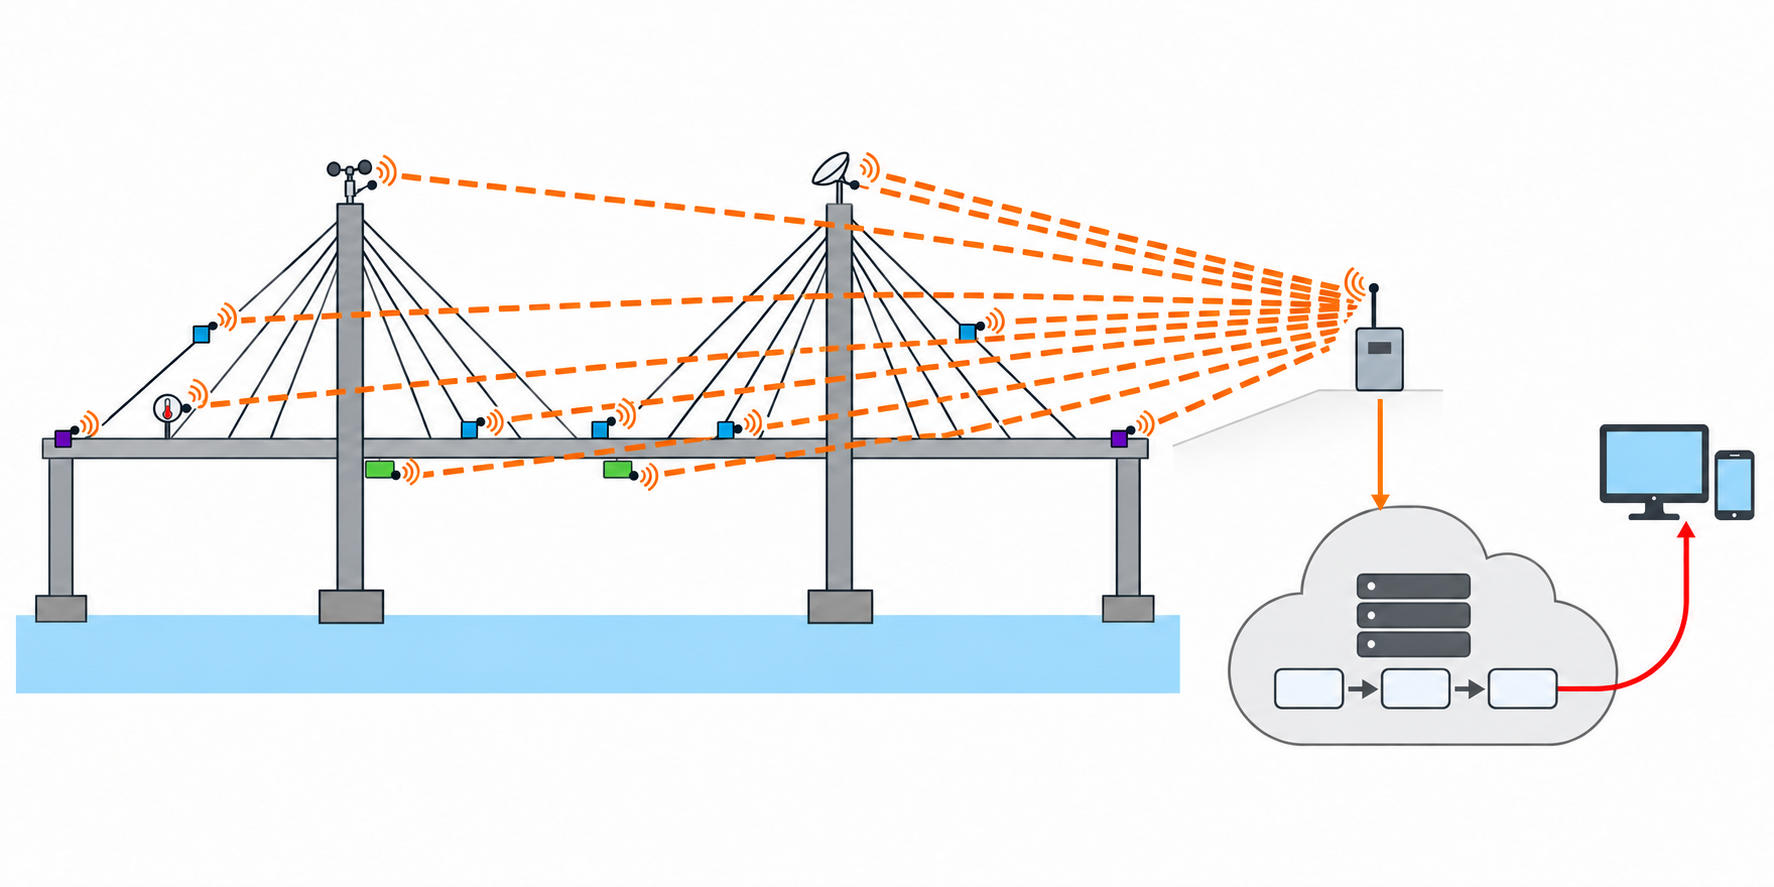
\includegraphics[width=\linewidth]{figures/ch11/ch11-06-v4-recovered.png}};
\begin{scope}[x={(img.south east)},y={(img.north west)}]
  \tikzset{
    lbl/.style={font=\sffamily\scriptsize,text=BookInk,fill=white,fill opacity=0.88,text opacity=1,inner sep=1.2pt,rounded corners=1pt,align=center},
    boxlbl/.style={font=\sffamily\tiny,text=BookInk,align=center,inner sep=0.5pt},
    ldr/.style={draw=BookInk!65,line width=0.45pt}
  }
  \node[lbl] (t1) at (0.11,0.77) {桥塔};
  \draw[ldr] (t1.east) -- (0.19,0.73);
  \node[lbl] (t2) at (0.33,0.76) {斜拉索（共 16 根）};
  \draw[ldr] (t2.south) -- (0.29,0.66);
  \node[lbl] (t3) at (0.56,0.42) {主梁};
  \draw[ldr] (t3.north) -- (0.56,0.49);
  \node[lbl,text=Ch11Orange!90!black] at (0.62,0.80) {无线传输链路};
  \node[lbl] (t5) at (0.86,0.64) {现场网关};
  \draw[ldr] (t5.west) -- (0.80,0.61);
  \node[lbl] at (0.80,0.45) {云端分析子系统};
  \node[boxlbl] at (0.738,0.224) {数据\\[-1pt]清洗};
  \node[boxlbl] at (0.798,0.224) {特征\\[-1pt]提取};
  \node[boxlbl] at (0.859,0.224) {阈值/\\[-1pt]异常判断};
  \node[lbl,text=Ch11Red,anchor=east] (t7) at (0.985,0.58) {预警通知管理人员\\[-1pt]{\tiny（需工程师复核）}};
  \draw[draw=Ch11Red,line width=0.45pt] (t7.south) -- (0.94,0.51);

  \draw[draw=BookRule,fill=BookPale!55,rounded corners=2pt,line width=0.4pt] (0.015,0.015) rectangle (0.985,0.115);
  \node[font=\sffamily\bfseries\tiny,text=BookInk,anchor=west] at (0.025,0.082) {传感器图例：};
  \filldraw[fill=Ch11Blue,draw=Ch11Gray,line width=0.4pt] (0.135,0.072) rectangle (0.147,0.092);
  \fill[black] (0.151,0.082) circle (0.0025);
  \node[font=\sffamily\tiny,text=BookInk,anchor=west] at (0.156,0.082) {加速度计（主梁 3 / 拉索 2）};
  \filldraw[fill=Ch11Green,draw=Ch11Gray,line width=0.4pt] (0.375,0.074) rectangle (0.393,0.090);
  \node[font=\sffamily\tiny,text=BookInk,anchor=west] at (0.398,0.082) {应变计（梁底 2）};
  \draw[Ch11Gray,line width=0.5pt] (0.535,0.070) -- (0.535,0.092);
  \draw[Ch11Gray,line width=0.5pt] (0.527,0.088) -- (0.543,0.088);
  \fill[Ch11Gray] (0.527,0.088) circle (0.003);
  \fill[Ch11Gray] (0.543,0.088) circle (0.003);
  \node[font=\sffamily\tiny,text=BookInk,anchor=west] at (0.548,0.082) {风速风向仪（左塔顶 1）};
  \draw[Ch11Gray,fill=white,line width=0.5pt] (0.715,0.084) ellipse (0.008 and 0.005);
  \draw[Ch11Gray,line width=0.5pt] (0.715,0.071) -- (0.715,0.080);
  \node[font=\sffamily\tiny,text=BookInk,anchor=west] at (0.727,0.082) {GNSS 天线（右塔顶 1）};
  \draw[Ch11Gray,fill=white,line width=0.5pt] (0.885,0.082) circle (0.006);
  \node[font=\sffamily\tiny,text=BookInk,anchor=west] at (0.894,0.082) {温度计（1）};

  \filldraw[fill=Ch11Purple,draw=Ch11Gray,line width=0.4pt] (0.028,0.030) rectangle (0.040,0.050);
  \node[font=\sffamily\tiny,text=BookInk,anchor=west] at (0.045,0.040) {位移计（两端 2）};
  \node[font=\sffamily\bfseries\tiny,text=BookInk,anchor=west] at (0.185,0.040) {连接线：};
  \draw[Ch11Gray,line width=0.6pt] (0.255,0.040) -- (0.285,0.040);
  \node[font=\sffamily\tiny,text=BookInk,anchor=west] at (0.290,0.040) {斜拉索（结构构件）};
  \draw[Ch11Orange,dashed,line width=1.1pt] (0.435,0.040) -- (0.470,0.040);
  \node[font=\sffamily\tiny,text=BookInk,anchor=west] at (0.475,0.040) {无线传输（传感器$\rightarrow$网关）};
  \draw[Ch11Orange,line width=1.1pt,-{Stealth[length=1.4mm]}] (0.665,0.040) -- (0.695,0.040);
  \node[font=\sffamily\tiny,text=BookInk,anchor=west] at (0.700,0.040) {广域网上传};
  \draw[Ch11Gray,line width=0.8pt,-{Stealth[length=1.3mm]}] (0.795,0.040) -- (0.820,0.040);
  \node[font=\sffamily\tiny,text=BookInk,anchor=west] at (0.825,0.040) {分析步骤};
  \draw[Ch11Red,line width=1.1pt,-{Stealth[length=1.4mm]}] (0.900,0.040) -- (0.930,0.040);
  \node[font=\sffamily\tiny,text=Ch11Red,anchor=west] at (0.935,0.040) {预警通知};
\end{scope}
\end{tikzpicture}
\caption{斜拉桥结构健康监测系统示意图（在 V4 底图上叠加 TikZ 标签与图例；教学用简化架构）。传感器布设于主梁、拉索与塔顶，数据经无线节点汇至现场网关，上传云端完成数据清洗、特征提取与阈值/异常判断，预警发送给管理人员并由工程师复核。图示不对应任何真实桥梁；实际系统常结合有线与无线传输，传感器数量与位置由具体设计决定。底图由图像模型生成，文字与图例以 TikZ 叠加；底图遗留偏差见表~\ref{tab:ch11-05}。}\label{fig:ch11-06}
\end{figure}

最后对照十项验收标准（F1--F10）完成整图复核（表~\ref{tab:ch11-05}）。如实列出底图尚未解决的局部偏差（拉索局部白隙、温度计内红色、云在网关下方、传感器图标偏小及待同行签字），才能明确正式投稿前在矢量软件里还需做哪几步收尾。

\begin{table}[htbp]\centering\footnotesize
\setlength{\tabcolsep}{3pt}
\renewcommand{\arraystretch}{1.15}
\caption{图~\ref{fig:ch11-06} 的十项整图核验记录。}\label{tab:ch11-05}
\begin{tabularx}{\linewidth}{@{}c>{\raggedright\arraybackslash}p{26mm}>{\raggedright\arraybackslash}p{16mm}Y>{\raggedright\arraybackslash}p{22mm}@{}}
\toprule
\textbf{\#} & \textbf{检查项} & \textbf{方法} & \textbf{实测结果与遗留偏差} & \textbf{结论} \\
\midrule
F1 & 双塔斜拉桥，无主缆/吊杆 & 目视 & 双塔斜拉桥侧视构型正确，无主缆或竖直吊杆 & 通过 \\
F2 & 拉索 16 根，均连塔与梁 & $200\%$ 计数 & 走向 $4+4+4+4=16$ 根，连塔与梁；但穿过图标与波纹处留有局部白隙 & 走向通过；断口待补线 \\
F3 & 12 个传感器类型与位置 & 对表计数 & $3+2+2+1+1+1+2=12$ 位置正确；温度计内部含红色，未精测同类色值 & 计数通过；温度计待去红 \\
F4 & L1--L4 方向与线型正确 & 逐条追踪 & 四类线语义方向正确，无越级直连；但云在网关下方使上传箭头朝下，局部有渐变 & 方向通过；上下布局有偏差 \\
F5 & 灰度下无线线与拉索可分 & 转灰度图 & 粗短虚线与细实线在灰度预览下可清楚区分 & 通过 \\
F6 & 底图无字，标签逐字比对 & $200\%$ 放大 & 底图零文字；TikZ 标签与图例逐字核对无误 & 通过 \\
F7 & $160\ \text{mm}$ 宽下图标 $\ge 2\ \text{mm}$、字 $\ge 6\ \text{pt}$ & 尺寸折算 & TikZ 文字 $\ge 6\ \text{pt}$；底图蓝方块折算约 $1.44\text{--}1.80\ \text{mm}$ 偏小 & 文字通过；小图标待放大 \\
F8 & 与 V2 相比无新意外变化 & 查修订表 & V4 相对 V2 未丢失或新增构件、传感器与箭头 & 通过 \\
F9 & 图注含简化与复核声明 & 读图注 & 已写明“教学用简化架构”与“预警由工程师复核” & 通过 \\
F10 & 结构工程同行复核签字 & 人工审阅 & 已完成作者核查；正式投稿前需结构工程同行复核签字 & 待同行签字 \\
\bottomrule
\end{tabularx}
\end{table}

\section{AI 在这一步能做什么与不能做什么}

修改与复核环节中 AI 与作者的分工汇总于表~\ref{tab:ch11-06}。

\begin{table}[htbp]\centering\footnotesize
\setlength{\tabcolsep}{3pt}
\renewcommand{\arraystretch}{1.15}
\caption{修改与复核环节中 AI 能做什么、不能做什么与作者要核对的内容。}\label{tab:ch11-06}
\begin{tabularx}{\linewidth}{@{}>{\raggedright\arraybackslash}p{18mm}YYY@{}}
\toprule
\textbf{环节} & \textbf{AI（\scidraw{} 等）能做} & \textbf{AI 不能做} & \textbf{作者要核对} \\
\midrule
理解意见 & 把一段口头意见改写成条目；按三层分类给出建议 & 判断哪条是科学错误（需领域知识与研究材料） & 每条问题能否定位到对象与位置；层级是否正确 \\
生成修改指令 & 把修改单条目改写成清楚的提示词 & 保证模型只执行这一条 & 指令包含“只改什么”和“保持不变”清单 \\
执行修改（图像） & 在 \scidraw{} 绘图中选历史图作参考并按指令多次迭代 & 对象锁定、区域保持；保证其他对象不变 & 每次修改后整图复核：对象计数、关系、文字、风格 \\
执行修改（数据图） & \scidraw{} 科学可视化可多轮对话修改，并恢复上一版或原版；由代码或配置重绘 & 判断修改后的统计表达是否仍正确 & 数据点、坐标轴、误差表达是否仍与数据一致 \\
比较版本 & （外部脚本）差异图、并排排版 & 产品内并排比较与命名（当前未提供，需下载后自行比较） & 人工按对象表计数；差异图只作辅助 \\
回退 & 重新选择历史中的某一版继续修改；数据图可一键恢复 & 自动判断哪一版是“正确基准” & 记录基准版本；在修订记录中写明“基于哪一版” \\
文字与精确样式 & — & 可靠拼写、精确色值与线型对齐 & 在排版层（TikZ/矢量软件）完成并逐字核对 \\
记录 & — & 自动生成可追溯的修订记录 & 每一版：基于、指令原文、目标修改、意外变化、复核结论、是否采用 \\
\bottomrule
\end{tabularx}
\end{table}

\section{本章检查清单}

\begin{itemize}
\item 每条意见都已翻译成“位置 + 现象”，并标注了层级（科学错误 / 阅读障碍 / 视觉一致性）。
\item 科学错误先于其他问题处理；科学错误多时选择重写输入而不是修补。
\item 修改单每条只说一件事，并写明“保持不变”的对象清单和核对方法。
\item 文字、精确色值、线型对齐类修改优先在排版层完成。
\item 每次生成式修改后，都按对象表与关系表**整图**复核，而不是只看改过的地方。
\item 与上一版并排比较；对象逐项计数；必要时用差异图辅助定位。
\item 发现连带变化后，回到上一个通过复核的版本，而不是在出错版本上叠加修改。
\item 同一修改两次仍有连带变化时，换路线（例如改在排版层完成）。
\item 修订记录中每一版都写明基于哪一版、指令原文、意外变化和是否采用；失败稿保留。
\item 终稿通过领域同行复核。
\end{itemize}

\section{练习}

\begin{enumerate}
\item \textbf{意见翻译（纸笔）。}拿出你最近收到的一条模糊意见（或用“这张图不够专业”），按本章三句追问，写出至少 6 条“位置 + 现象”问题，标注层级并排序，说明哪两条你会合并到同一次修改、哪一条要放到排版层处理。
\item \textbf{\scidraw{} 实操：连带变化实验。}在 \scidraw{} 绘图中生成或上传一张你自己的示意图作为 V2，选择它作为参考图，只要求改一处线型或颜色。生成后与 V2 并排，按你事先写好的对象表逐项计数，记录目标修改是否完成、有没有连带变化；然后回到 V2，加上保留清单重做一次，比较两次结果。把两次的记录整理成表~\ref{tab:ch11-04} 格式的修订记录。
\item \textbf{数据图对照。}在 \scidraw{} 科学可视化（\sdtool{sci-vis}）中上传一份公开数据或模拟数据，生成一张图后连续做三次修改（例如改配色、改坐标轴范围、改图例位置），再恢复到上一版和原版。写一段 200 字说明：数据图的修改和恢复与示意图的生成式修改有什么不同；为什么两者都仍需要整图复核。
\end{enumerate}

\section*{参考文献}

\begin{itemize}
\item Farrar CR, Worden K. An introduction to structural health monitoring. \textit{Philosophical Transactions of the Royal Society A}. 2007;365(1851):303--315. doi:10.1098/rsta.2006.1928
\item Kim S, Pakzad S, Culler D, Demmel J, Fenves G, Glaser S, Turon M. Health monitoring of civil infrastructures using wireless sensor networks. In: \textit{Proceedings of the 6th International Conference on Information Processing in Sensor Networks (IPSN '07)}. ACM; 2007:254--263. doi:10.1145/1236360.1236395
\item Ko JM, Ni YQ. Technology developments in structural health monitoring of large-scale bridges. \textit{Engineering Structures}. 2005;27(12):1715--1725. doi:10.1016/j.engstruct.2005.02.021
\item Lynch JP, Loh KJ. A summary review of wireless sensors and sensor networks for structural health monitoring. \textit{The Shock and Vibration Digest}. 2006;38(2):91--128. doi:10.1177/0583102406061499
\item Rougier NP, Droettboom M, Bourne PE. Ten simple rules for better figures. \textit{PLoS Computational Biology}. 2014;10(9):e1003833. doi:10.1371/journal.pcbi.1003833
\item Wong B. Simplify to clarify. \textit{Nature Methods}. 2011a;8(8):611. doi:10.1038/nmeth.1660
\item Wong B. Points of view: Color blindness. \textit{Nature Methods}. 2011b;8(6):441. doi:10.1038/nmeth.1618
\end{itemize}

% TODO: figures/ch11/ch11-03-v2-brief.png 与 figures/ch11/ch11-06-v4-recovered.png 尚存 4 处已知底图偏差（云在网关下方、温度计含红色、160 mm 宽下蓝方块约 1.44-1.80 mm 偏小、部分拉索穿过图标处有窄白隙），正文与表 11-3、11-4、11-5 已如实说明。
% TODO: figures/ch11/ch11-05-diff-and-count-zh.pdf 仅含第 7 章差异热图行与两案例计数表（表格末行底边略裁切）；若后续重跑脚本加入本章 V2/V3 差异热图行，需微调图 11-5 图注。
% TODO: figures/ch11/ch11-08-version-tree-zh.tex 图中节点 V3 文字为“连带变化（不采用）”，正文与图 11-8 图注已说明该分支用于示意出现连带变化时的回退逻辑。
